\documentclass[14pt,a4paper]{extarticle} 
\usepackage[T2A]{fontenc}
\usepackage[utf8]{inputenc}
\usepackage[top=0.78in, bottom=0.78in, right=0.59in, includefoot]{geometry}
\usepackage[english, russian]{babel} % Подключение русского языка
\usepackage{indentfirst} % Абзацы
\usepackage{amsmath, amsfonts, amssymb, amsthm, mathtools}
\usepackage[T2A]{fontenc}
\usepackage[utf8]{inputenc}

\usepackage{titlesec}
% Центрирование \section
\titleformat{\section} % Команда для настройки \section
{\centering\normalfont\Large\bfseries} % Стиль: центрирование, крупный шрифт, жирный
{\thesection} % Номер раздела
{1em} % Расстояние между номером и заголовком
{} % Дополнительный код после заголовка

\usepackage[hidelinks]{hyperref} % подключение ссылок
\usepackage{nameref} 
\usepackage{csquotes} 

\usepackage{hyphsubst} % Этот пакет позволяет настраивать правила переноса слов
\usepackage{minted} % Используется для форматирования и подсветки синтаксиса кода

\usepackage{titleps} % создание линий для колонтитулов
\newpagestyle{main}{
	% \setfootrule{0.4pt}
	\setfoot{}{\thepage}{}
}

\pagestyle{main}

%\linespread{1} % Отступы между строками
%\setlength{\parindent}{20pt}
%\setlength{\parskip}{10pt}

% Создание теорем, определений и прочего. Можно поменять стиль, сделать разное оформление к каждому разделу, но придется дописывать преамбулу
\usepackage{amsthm}
\theoremstyle{plain}
\newtheorem{theorem}{Теорема}
\newtheorem*{definition}{Определение}
\newtheorem*{corollary}{Следствие}
\newtheorem*{note}{Замечание}


\usepackage{tocloft} % Позволяет настраивать внешний вид оглавления (table of contents), списка фигур (list of figures) и списка таблиц (list of tables)
\renewcommand{\cftsecleader}{\cftdotfill{\cftdotsep}} % Заполнение пробелов между заголовками секций и номерами страниц в оглавлении
%\renewcommand{\thesection}{\arabic{section}.} % Переопределяет формат отображения номера секции. В данном случае, номера секций будут отображаться в арабском формате (1, 2, 3 и т.д.) и будут следовать с точкой (используйте, если у вас нет поздразделов, иначе у них будет писать 1..1 и так далее)

%Создание изображений
\usepackage{graphicx} % Вставка изображений
%\usepackage{float} % "Плавающие" картинки
\usepackage{wrapfig} % Обтекание фигур (таблиц, картинок и прочего)
\usepackage{placeins} % Этот пакет управляет размещением плавающих объектов (таких как рисунки и таблицы) в документе
\usepackage[dvipsnames]{xcolor} % Предоставляет расширенные возможности работы с цветами
\usepackage{caption} % Используется для настройки внешнего вида подписей к рисункам и таблицам
\captionsetup[figure]{name=Рисунок}
\DeclareCaptionLabelSeparator{dash}{ --- } % Эта команда определяет разделитель между названием (например, "Рисунок") и текстом подписи
\captionsetup{labelsep=dash} % Эта команда применяет ранее определенный разделитель (в данном случае dash) ко всем подписям в документе

% Для таблиц
\usepackage[raggedrightboxes]{ragged2e}
\usepackage{makecell} 
\usepackage{tabularx}
\usepackage{enumitem} % Пакет для гибкой настройки списка
\usepackage{multicol}
\usepackage{multirow} 
\usepackage{booktabs}
\usepackage{float}
\usepackage{array}  
\usepackage{longtable}
\usepackage{pdflscape}
% Создание листинга программы
\usepackage{listings}
\usepackage{xcolor}


\lstset{
	language=C++,
	basicstyle=\ttfamily\scriptsize,
	keywordstyle=\color{blue}\bfseries,
	commentstyle=\color{green!60!black},
	stringstyle=\color{red},
	numbers=left,
	frame=none,
}



\newcommand{\mytitlepage}{
	\thispagestyle{empty}
	
	\centerline{\textbf{Министерство науки и высшего образования РФ}}
	\centerline{\textbf{Федеральное государственное бюджетное образовательное}}
	\centerline{\textbf{учреждение высшего образования}}
	\centerline{\textbf{<<Уфимский университет науки и технологий>>}}
	\vspace{5mm}
	\centerline{\textbf{Кафедра:} Высокопроизводительных вычислений и дифференциальных}
	\centerline{уравнений}
	
	
	\vspace{40mm}
	
	\centerline{\textbf{\makecell{МОДЕЛИРОВАНИЕ ДВУМЕРНЫХ\\ДИФФУЗИОННЫХ ПРОЦЕССОВ\\МЕТОДОМ НЕПРЕРЫВНЫХ\\СЛУЧАЙНЫХ БЛУЖДАНИЙ }}} % Написать все название капсом
	\vspace{5mm}
	\centerline{{\textbf{ОТЧЕТ}}}
	\vspace{2mm}
	\centerline{к лабораторной работе №4 по дисциплине}
	\vspace{2mm}
	\centerline{<<Математическое моделирование>>} % Написать название дисциплины
	%\vspace{4mm}
	%\centerline{\textbf{3952.236108.000 ПЗ}} % Посередине шифр ABCDEF
	% A - тип работы, где 2 - курсовой проект, 3 - курсовая работа (оставляем 2)
	% BС - код дисциплины, (состоит из кода учебной программы 3 и номера семестра)
	% D - обозначение группы: 1 у ПМ, 2 у Мкн
	% EF - номер в списке группы по журналу
	\vspace{30mm}
	% Указать группу, прописать фамилии и инициалы в таблице
	\begin{center}
		\bgroup
		\def\arraystretch{1.4}
		\setlength{\tabcolsep}{12pt}
		\begin{tabular}{|c|c|c|c|c|}
			\hline
			\makecell{Группа\\МКН-418Б} & Фамилия И.\ О. & Подпись & Дата & Оценка \\
			\hline
			Студент & Халитова А.А. &  &  & \\
			\hline
			Принял & Феоктистов Б.А. &  &  & \\
			\hline
		\end{tabular}
		\egroup
	\end{center}
	\vspace{40mm}
	\centerline{Уфа 2026} % Поменять год 
	\clearpage
}

\begin{document}
	\mytitlepage
	\tableofcontents
	\newpage
	
	\textbf{Цель работы:} получить навык статистического моделирования диффузионных процессов методом случайных блужданий.
	
	\newpage
	
	\section{Теоретическая часть}
	
	Рассматривается случайный процесс движения диффундирующей частицы на плоскости. В начальный момент времени частица находится в начале координат. Затем частица осуществляет «прыжок» на случайную величину $l$, подчиняющуюся заданному закону распределения с плотностью вероятности $f(l)$. Направление прыжка выбирается произвольно из четырех возможных: влево, вправо, вверх или вниз. На следующем шаге процесс повторяется с новым случайным значением $l$. Частица должна выполнить $N$ «прыжков». Весь процесс необходимо повторить для $M$ частиц.
	
	Вычислить функции распределения частиц $P_N(x)$, $P_N(y)$ по двум координатным направлениям, и рассчитать значения:
		
	\begin{equation}
		\centering
		\langle x_N \rangle = \dfrac{1}{M} \sum_{i = 1}^{M} x_i, \quad
		\langle y_N \rangle = \dfrac{1}{M} \sum_{i = 1}^{M} y_i, \quad
		\langle R_N \rangle = \sqrt{\langle x_N \rangle^2 + \langle y_N \rangle^2},
		\nonumber
	\end{equation}
	где $(x_i,y_i)$ - координата $i$-й частицы после $N$ прыжков. 
	
	Также вычисляются параметры:
	
	\begin{equation}
		\langle x_N^2 \rangle = \dfrac{1}{M} \sum_{i = 1}^{M} x_i^2, \quad
		\langle y_N^2 \rangle = \dfrac{1}{M} \sum_{i = 1}^{M} y_i^2, \quad
		\nonumber
	\end{equation}
	\begin{equation}
		\langle \Delta x_N^2 \rangle = \langle x_N^2 \rangle - \langle x_N \rangle^2, \quad
		\langle \Delta y_N^2 \rangle = \langle y_N^2 \rangle - \langle y_N \rangle^2,
		\nonumber
	\end{equation}
	как функции $N$. После этого находится средний квадрат полного смещения частиц:
	
	\begin{equation}
		\langle \Delta R_N^2 \rangle = \langle \Delta x_N^2 \rangle + \langle \Delta y_N^2 \rangle.
		\nonumber
	\end{equation}
	
	Для больших значений $N$ выполнить аппроксимацию этой величины степенной зависимостью
	
	\begin{equation}
		\langle \Delta R_N^2 \rangle \approx \mu  N^{\nu}.
		\label{min_squares_condition}
	\end{equation}
	
	В зависимости от найденного значения показателя $\nu$ сделать вывод о близости асимптотического распределения к нормальному закону.
	
	Все расчеты выполнить для значений функции плотности распределения вероятности длины прыжка, указанной в индивидуальном задании.
	При этом постоянная $A$ находится из условия:
	
	\begin{equation}
		\int_{0}^{\infty} f(l)dl =1.
		\label{a_condition}
	\end{equation}
	
	Для построения генератора случайных чисел, подчиняющихся заданной плотности распределения $f(l)$, использовать формулу:
	
	\begin{equation}
		l = F^{-1}(r),
		\nonumber
	\end{equation}
	где $r$ – равномерно распределенная на отрезке $[0,1]$ случайная величина и
	
	\begin{equation}
		F(l) = \int_{0}^{l} f(x) dx.
		\nonumber
	\end{equation}
	
	\section{Практическая часть}
	
	\subsection{Построение обратной функции}
	
	Практическая часть решается согласно варианту №7.
	
	Функция плотности распределения вероятности длины прыжка:
	
	\begin{equation}
		f(l) = \dfrac{Al^2}{l^6+1}.
		\label{ifit_func}
	\end{equation}
	
	Интеграл функции~\eqref{ifit_func} равен:
	
	\begin{equation}
		F(l) = \dfrac{A}{3} \arctg(l^3).
		\nonumber
	\end{equation}
	
	Их выражения ~\eqref{a_condition}:
	
	\begin{equation}
		A = \dfrac{6}{\pi}.
		\nonumber
	\end{equation}
	
	Тогда обратная фунция:
	
	\begin{equation}
		l = F^{-1}(r) = \sqrt[3]{\tg (\dfrac{\pi r}{2})}.
	\end{equation}
	
	\subsection{Моделирование движения частиц}
	
	Рассмотрим систему из частиц численности $M \in $ {$10^2$, $10^3$, $10^4$}. Для каждой величины M смоделируем траектории на протяжении $N$ шагов, где параметр $N$ принимает значения:
	\[
	N = 500, 1000, \ldots, 5000.
	\]

	\begin{figure}[H]
		\centering
		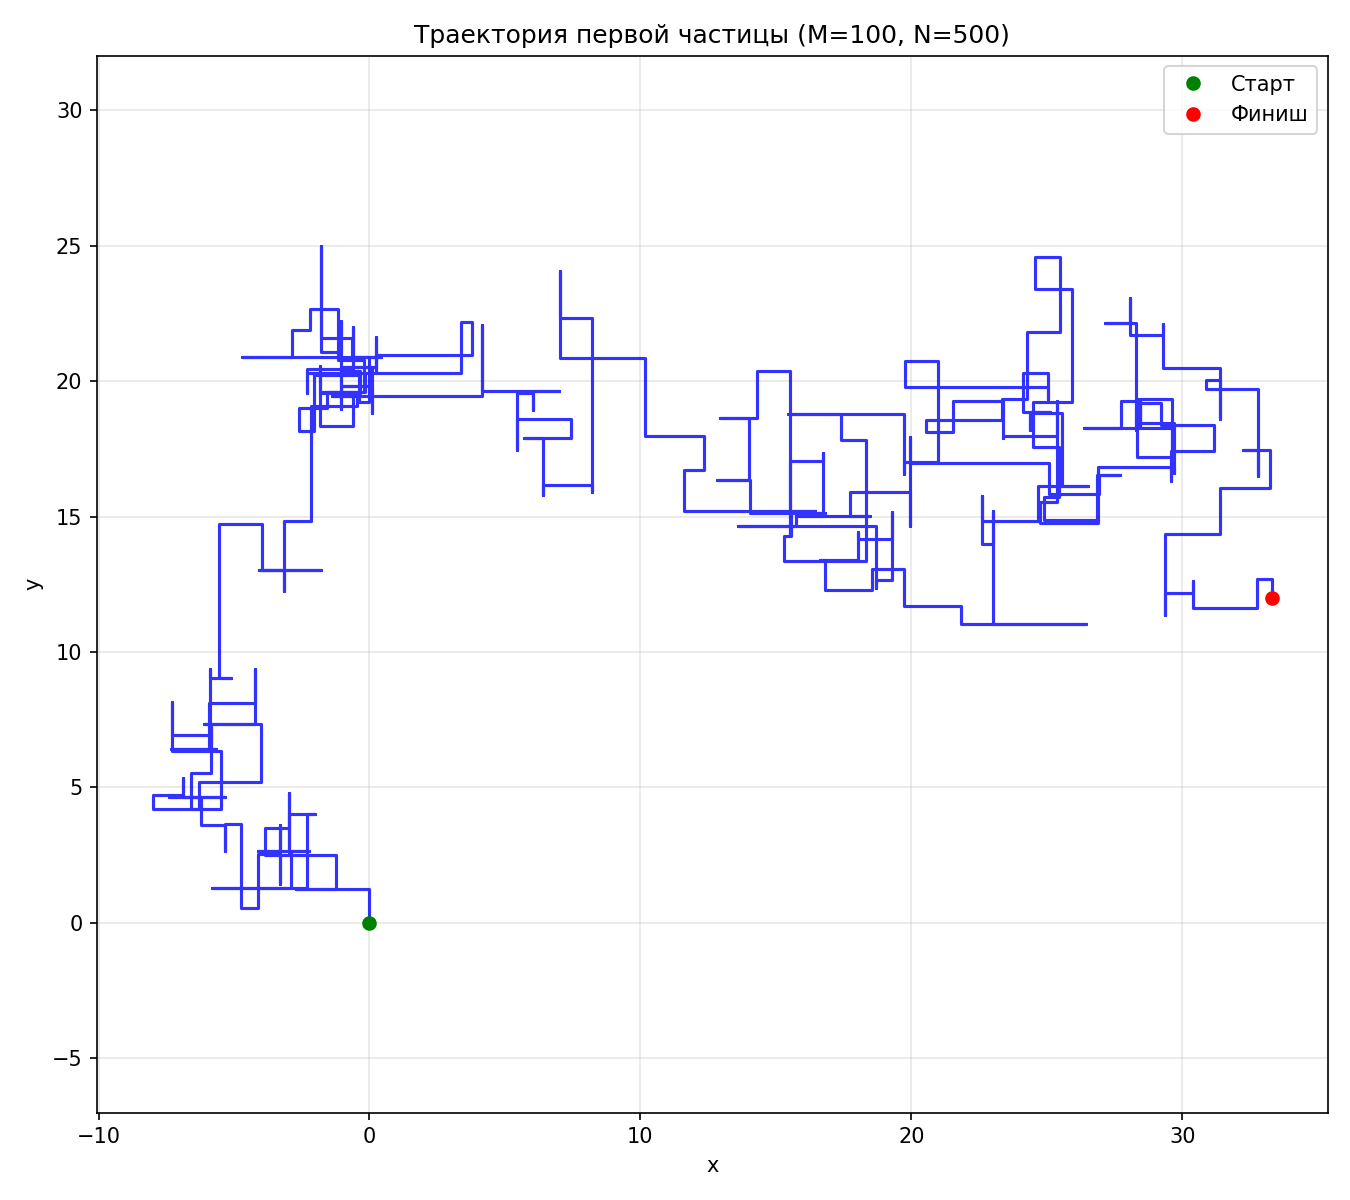
\includegraphics[width=0.7\linewidth]{../out/trajectory_M100_N500}
		\caption{ Траектория движения первой точки M = 100, N = 500}
		\label{fig:trajectorym100n500}
	\end{figure}
	
	\begin{figure}[H]
		\centering
		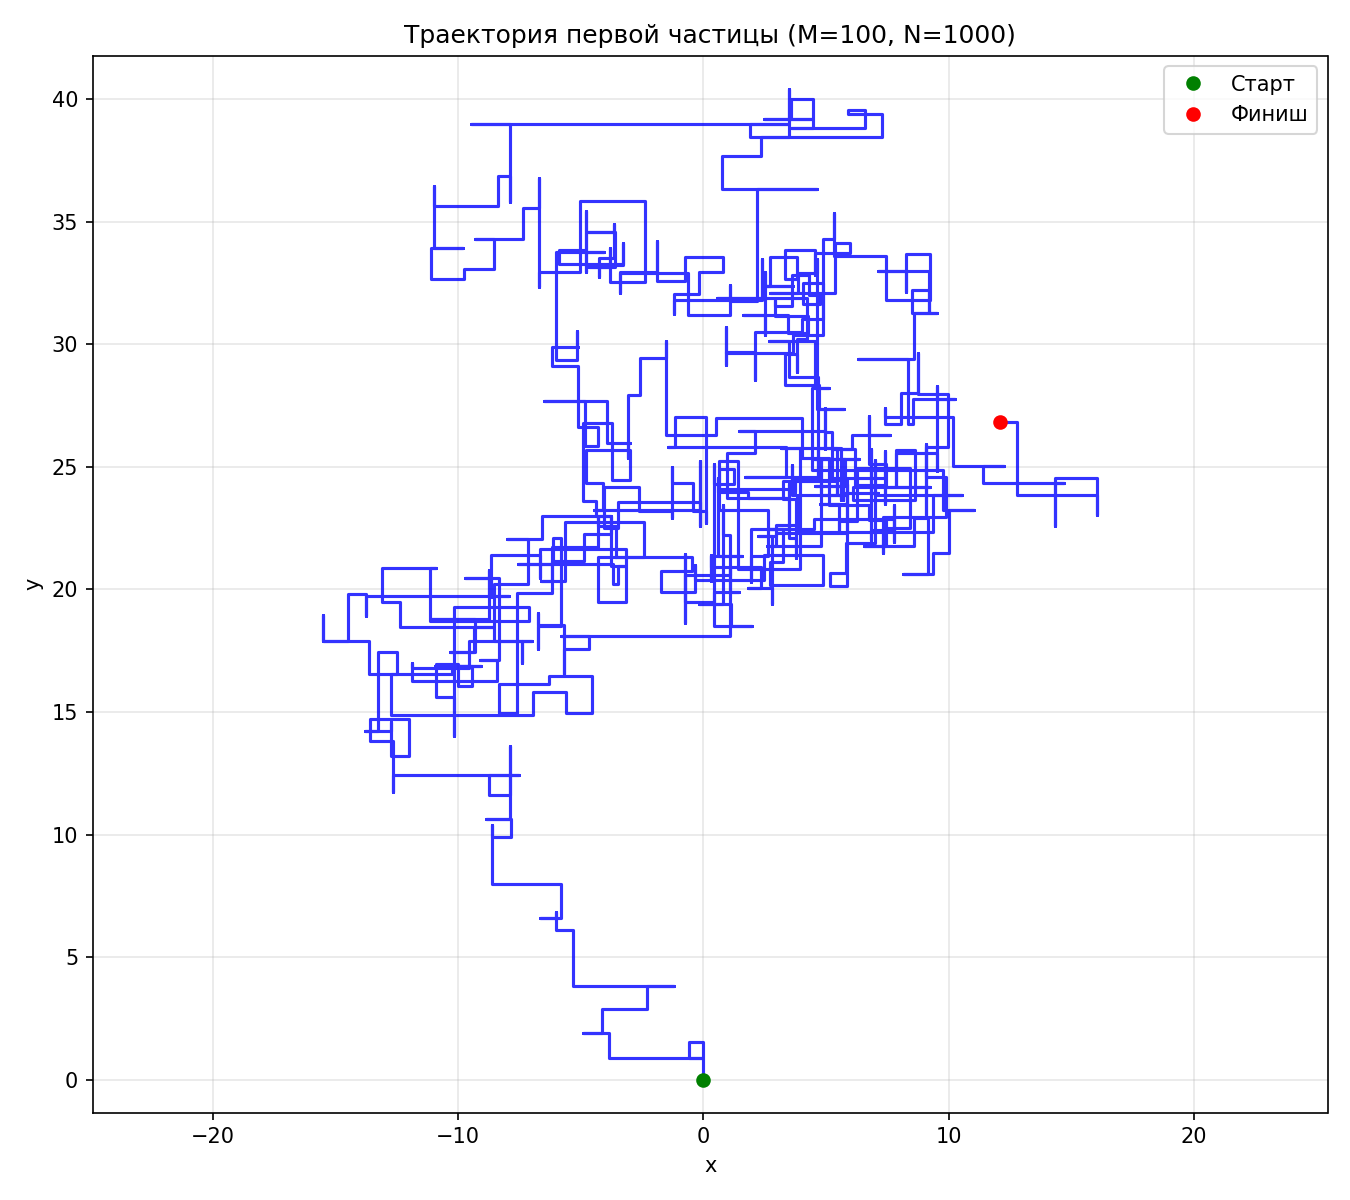
\includegraphics[width=0.7\linewidth]{../out/trajectory_M100_N1000}
		\caption{ Траектория движения первой точки M = 100, N = 1000}
		\label{fig:trajectorym100n1000}
	\end{figure}
	
	\begin{figure}[H]
		\centering
		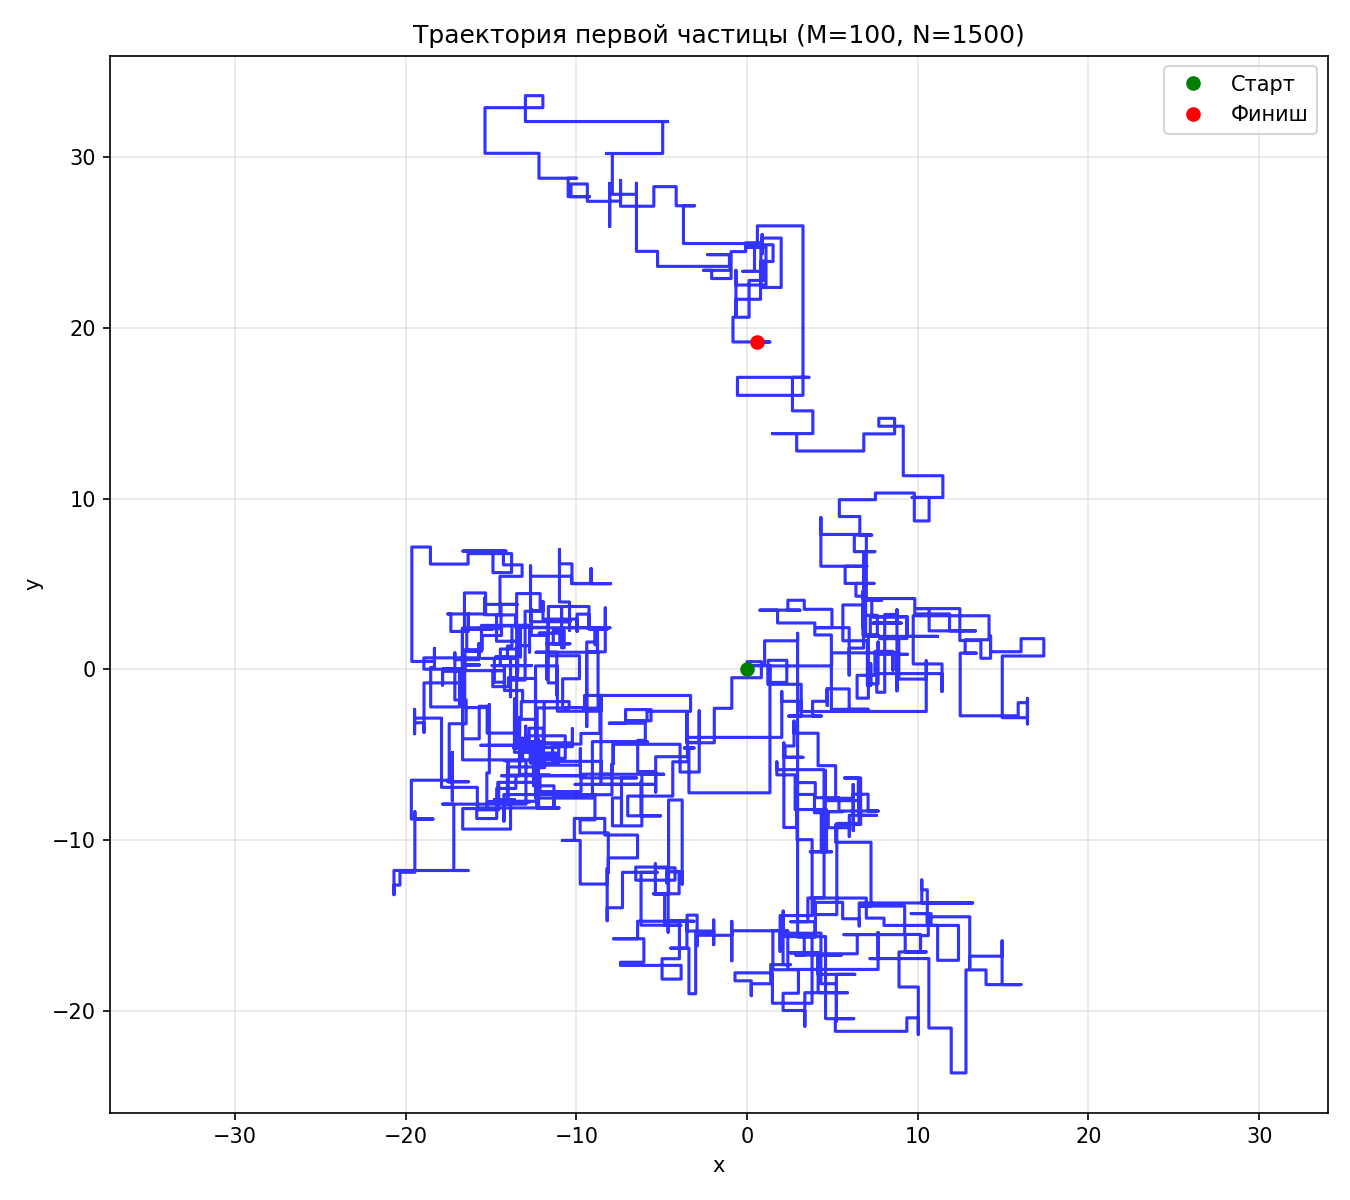
\includegraphics[width=0.7\linewidth]{../out/trajectory_M100_N1500}
		\caption{ Траектория движения первой точки M = 100, N = 1500}
		\label{fig:trajectorym100n1500}
	\end{figure}
	
	\begin{figure}[H]
		\centering
		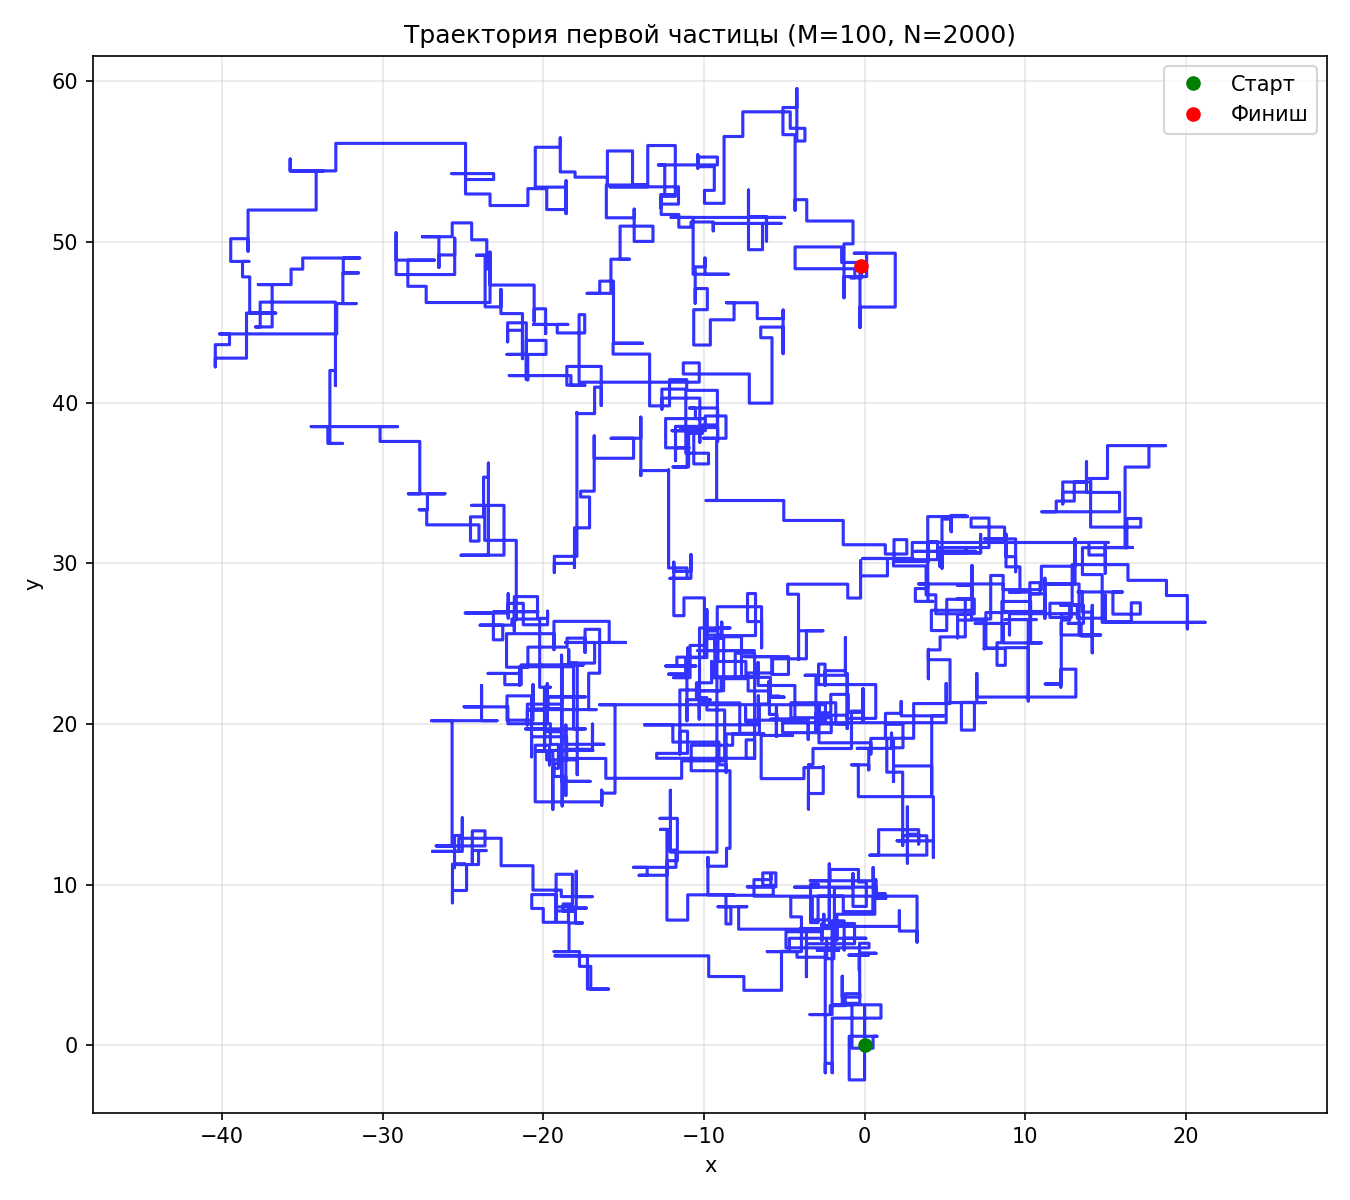
\includegraphics[width=0.7\linewidth]{../out/trajectory_M100_N2000}
		\caption{ Траектория движения первой точки M = 100, N = 2000}
		\label{fig:trajectorym100n2000}
	\end{figure}
	
	\begin{figure}[H]
		\centering
		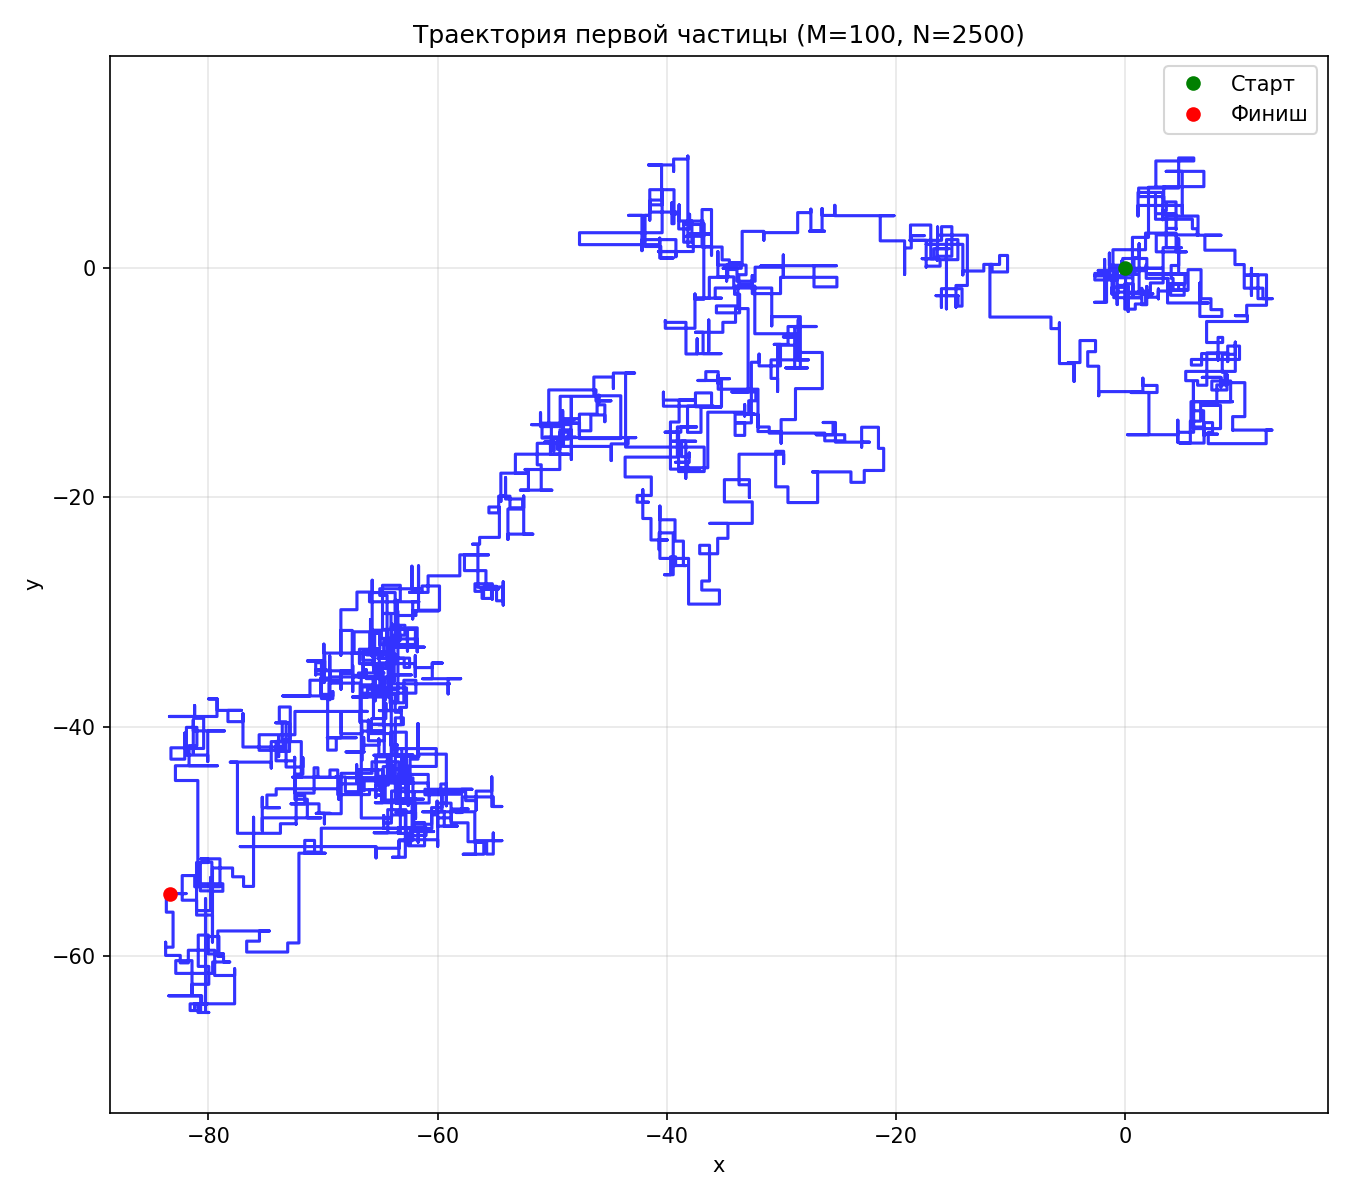
\includegraphics[width=0.7\linewidth]{../out/trajectory_M100_N2500}
		\caption{ Траектория движения первой точки M = 100, N = 2500}
		\label{fig:trajectorym100n2500}
	\end{figure}
	
	\begin{figure}[H]
		\centering
		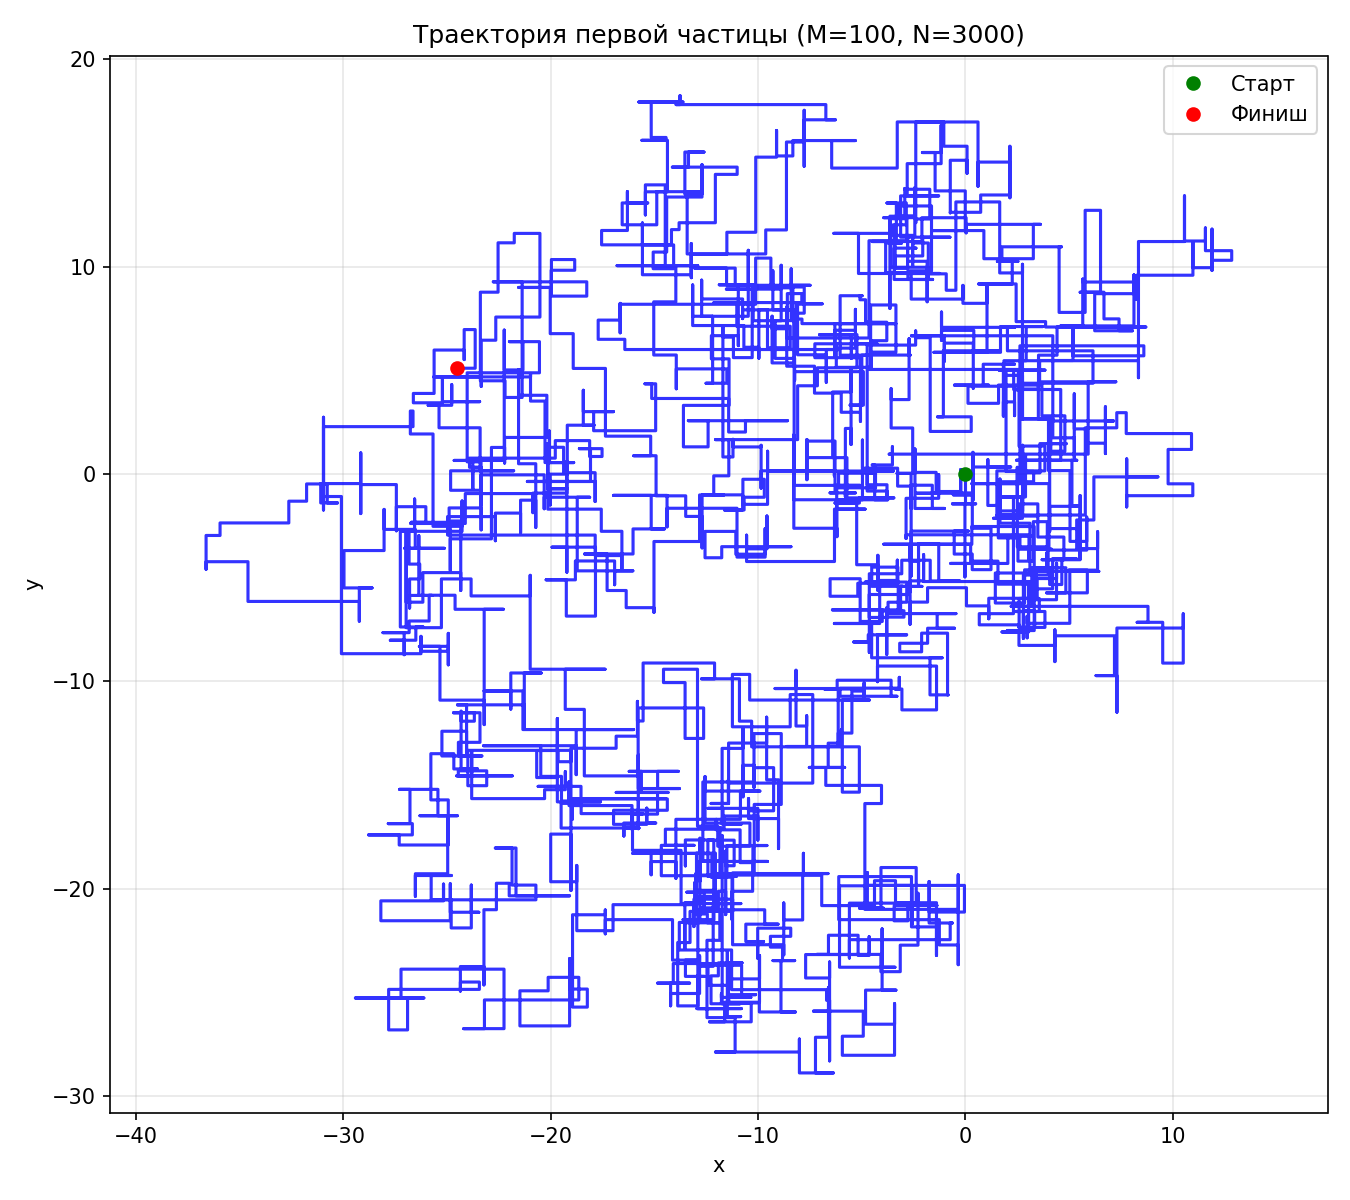
\includegraphics[width=0.7\linewidth]{../out/trajectory_M100_N3000}
		\caption{ Траектория движения первой точки M = 100, N = 3000}
		\label{fig:trajectorym100n3000}
	\end{figure}
	
	\begin{figure}[H]
		\centering
		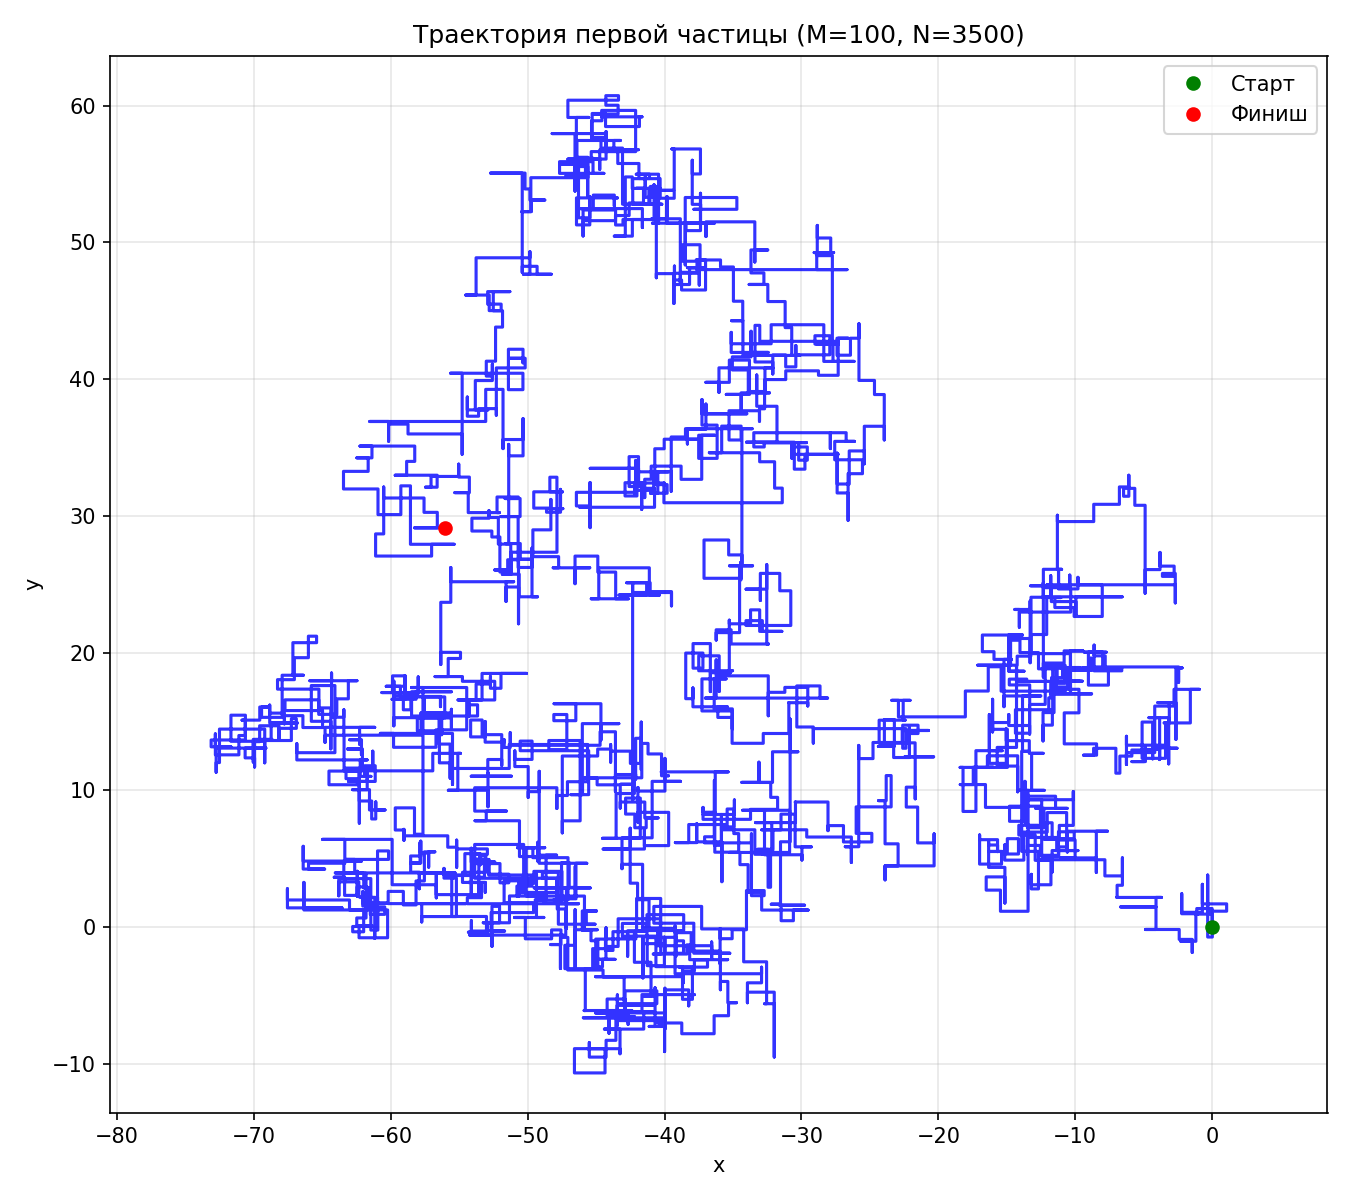
\includegraphics[width=0.7\linewidth]{../out/trajectory_M100_N3500}
		\caption{ Траектория движения первой точки M = 100, N = 3500}
		\label{fig:trajectorym100n3500}
	\end{figure}
	
	\begin{figure}[H]
		\centering
		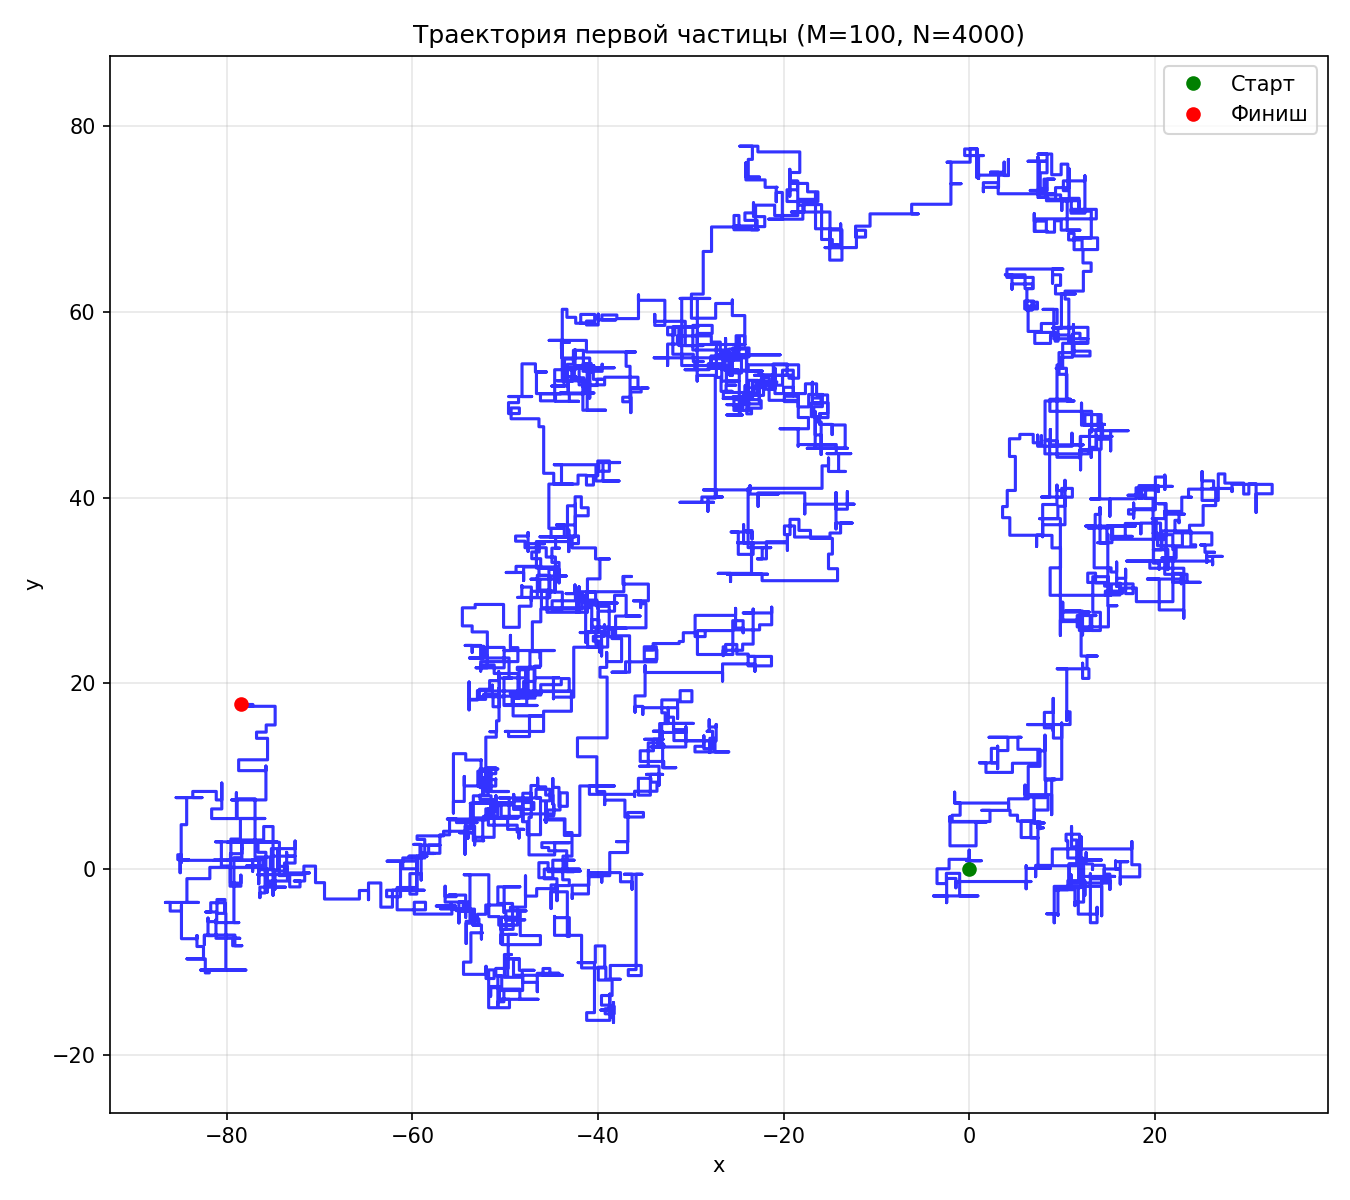
\includegraphics[width=0.7\linewidth]{../out/trajectory_M100_N4000}
		\caption{ Траектория движения первой точки M = 100, N = 4000}
		\label{fig:trajectorym100n4000}
	\end{figure}
	
	\begin{figure}[H]
		\centering
		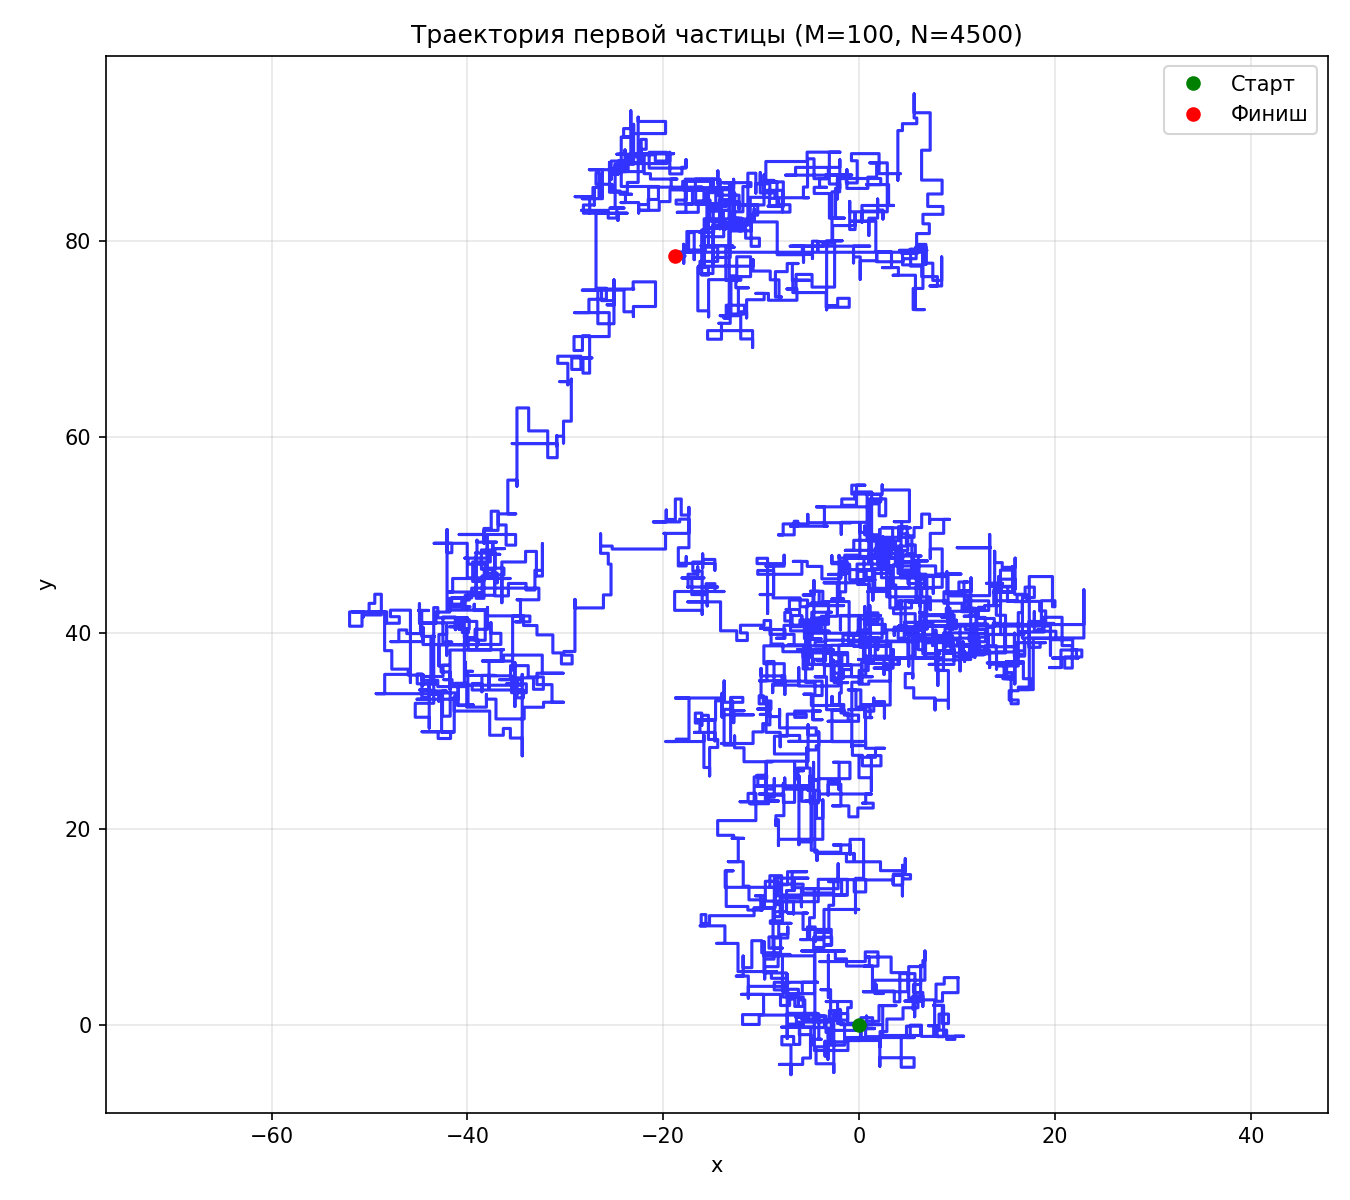
\includegraphics[width=0.7\linewidth]{../out/trajectory_M100_N4500}
		\caption{ Траектория движения первой точки M = 100, N = 4500}
		\label{fig:trajectorym100n4500}
	\end{figure}
	
	\begin{figure}[H]
		\centering
		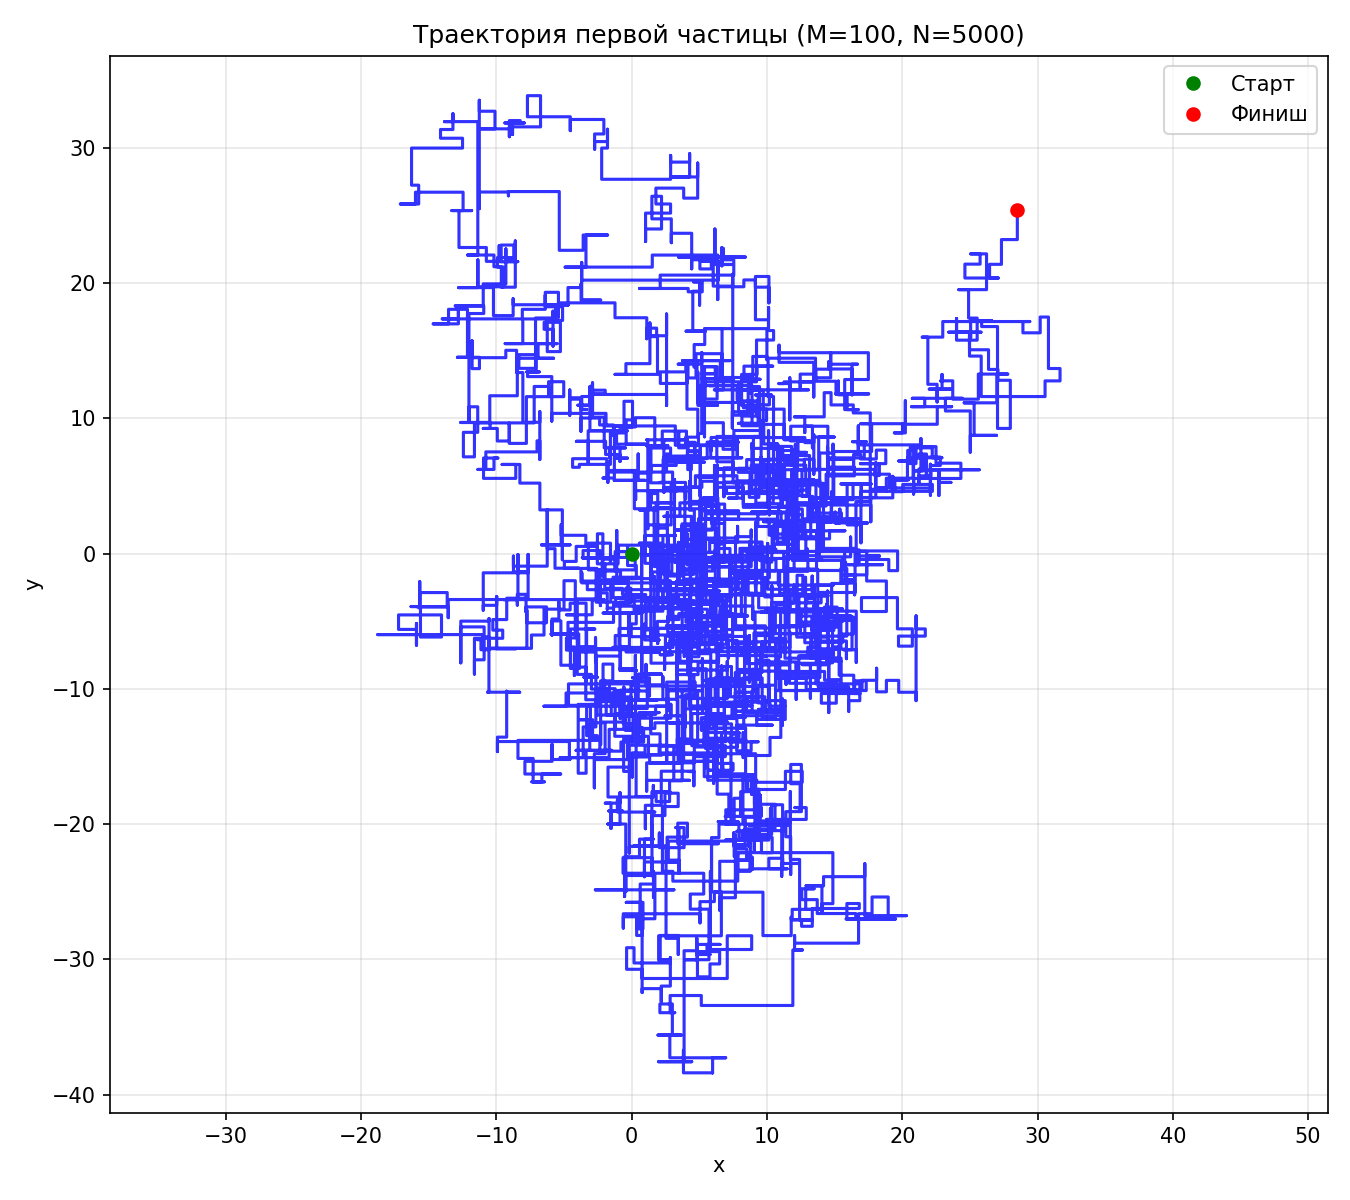
\includegraphics[width=0.7\linewidth]{../out/trajectory_M100_N5000}
		\caption{ Траектория движения первой точки M = 100, N = 5000}
		\label{fig:trajectorym100n5000}
	\end{figure}
	
	\subsection{Рассчитанные параметры}
	
	Для каждого количества частиц рассчитаем значения мат ожидания и вариации.
	
	\begin{figure}[H]
		\centering
		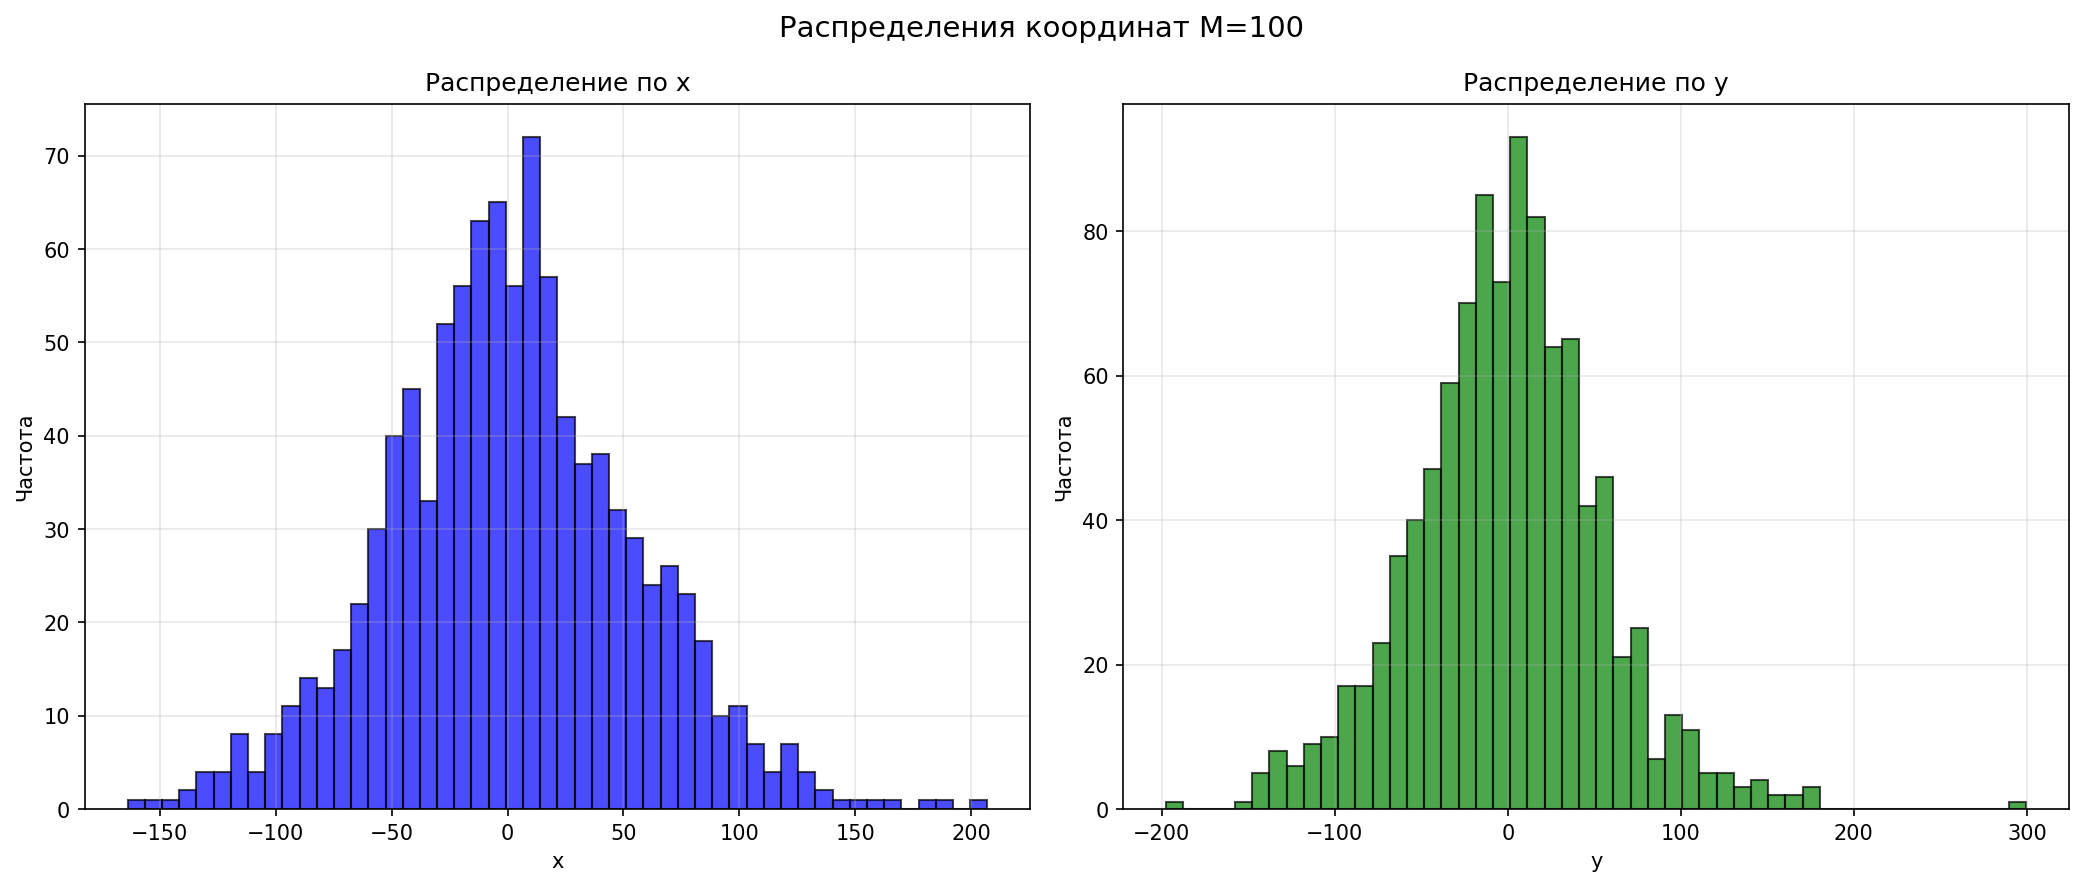
\includegraphics[width=1.0\linewidth]{../out/histograms_M100}
		\caption{Гистограмма распределения M = 100}
		\label{fig:histogramsm100}
	\end{figure}
	
	\begin{figure}[H]
		\centering
		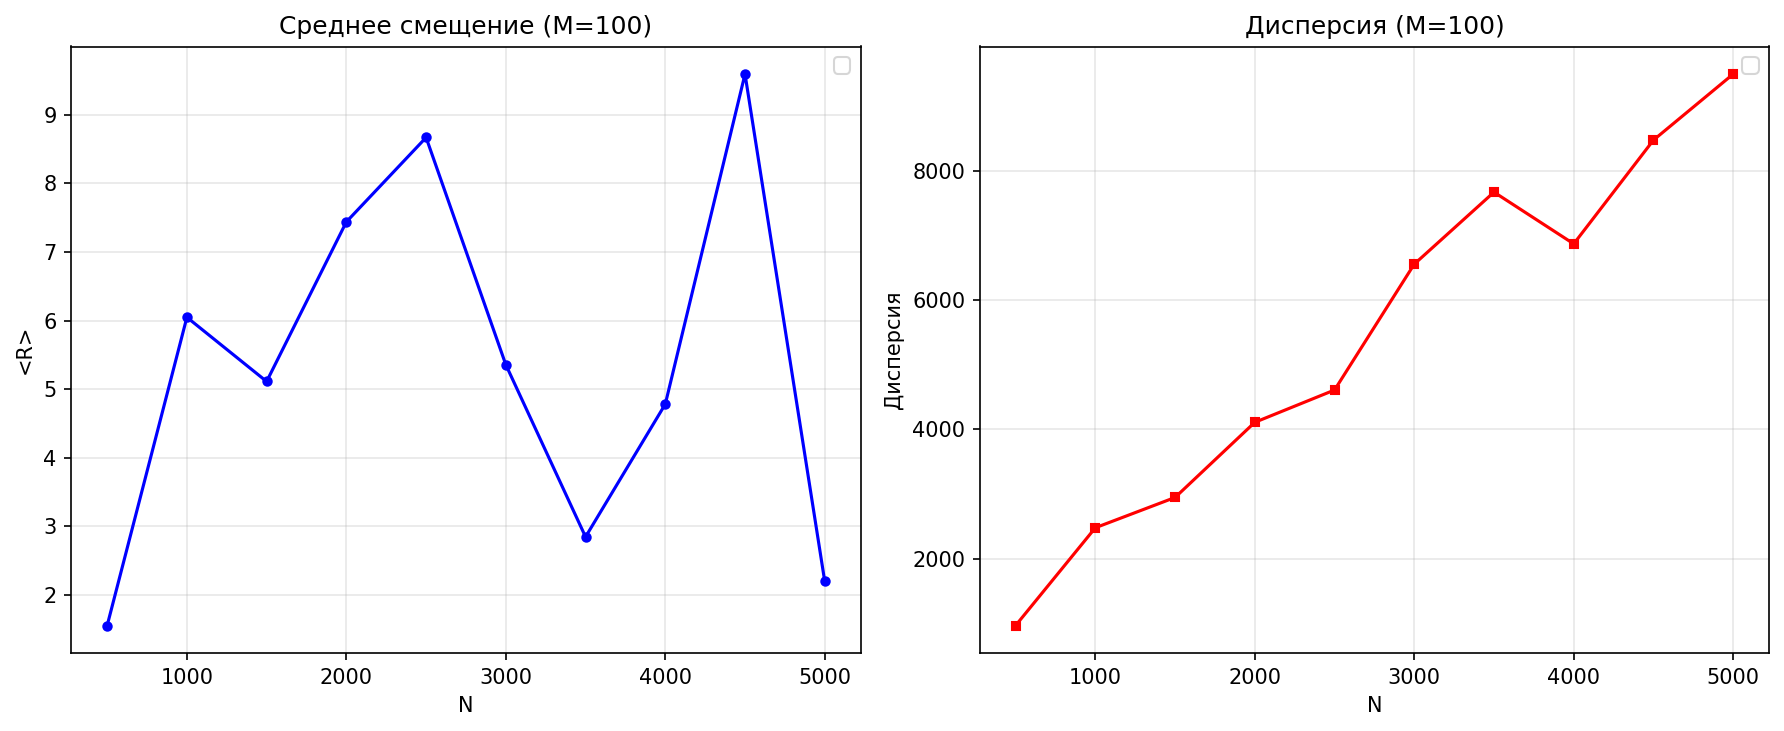
\includegraphics[width=1.0\linewidth]{../out/statistics_M100}
		\caption{Статистика для распределения M = 100}
		\label{fig:statisticsm100}
	\end{figure}
	
	\begin{figure}[H]
		\centering
		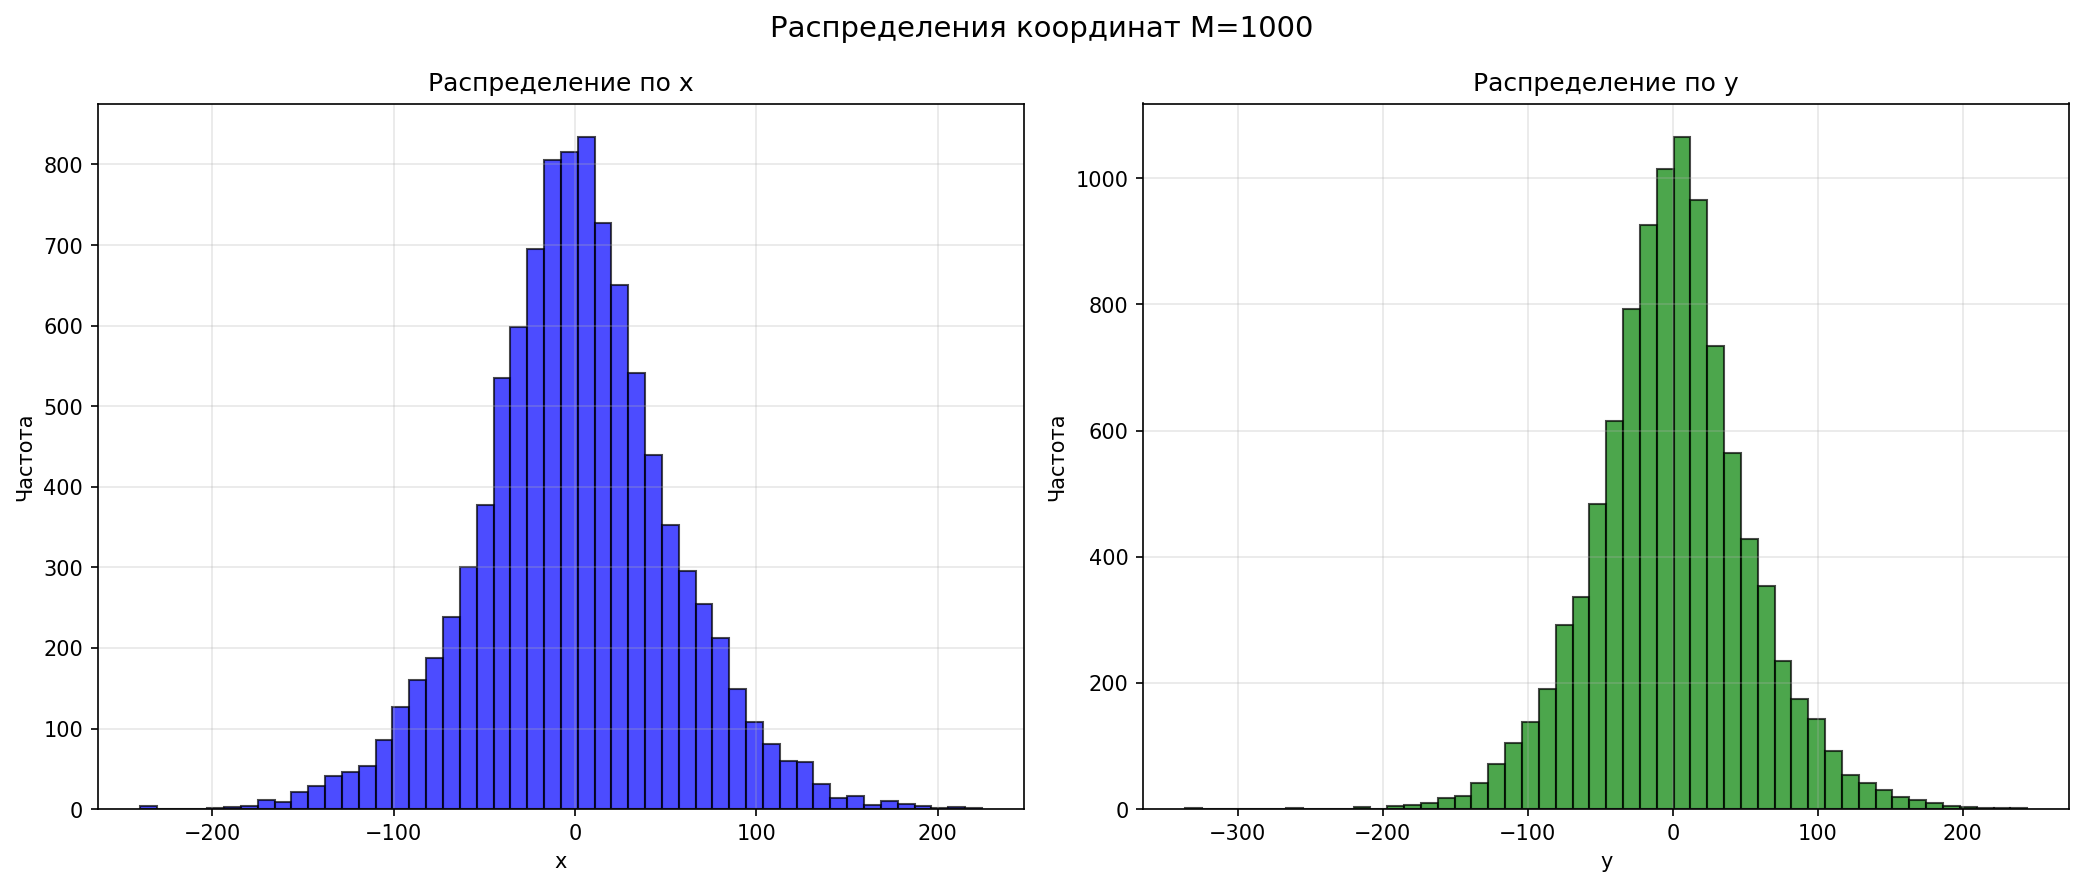
\includegraphics[width=1.0\linewidth]{../out/histograms_M1000}
		\caption{Гистограмма распределения M = 1000}
		\label{fig:histogramsm1000}
	\end{figure}
	
	\begin{figure}[H]
		\centering
		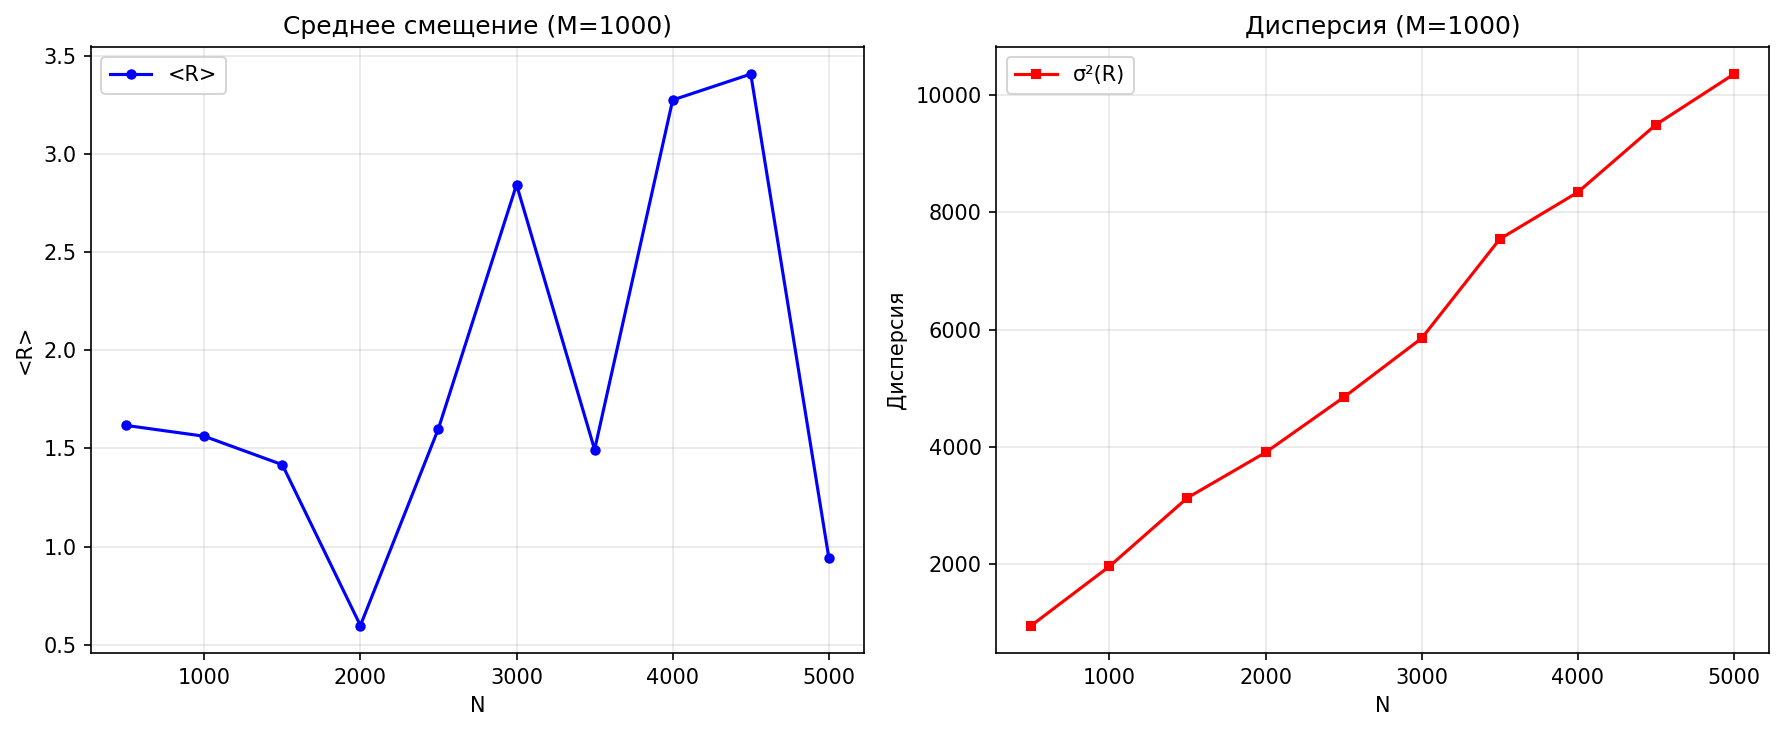
\includegraphics[width=1.0\linewidth]{../out/statistics_M1000}
		\caption{Статистика для распределения M = 1000}
		\label{fig:statisticsm1000}
	\end{figure}
	
	\begin{figure}[H]
		\centering
		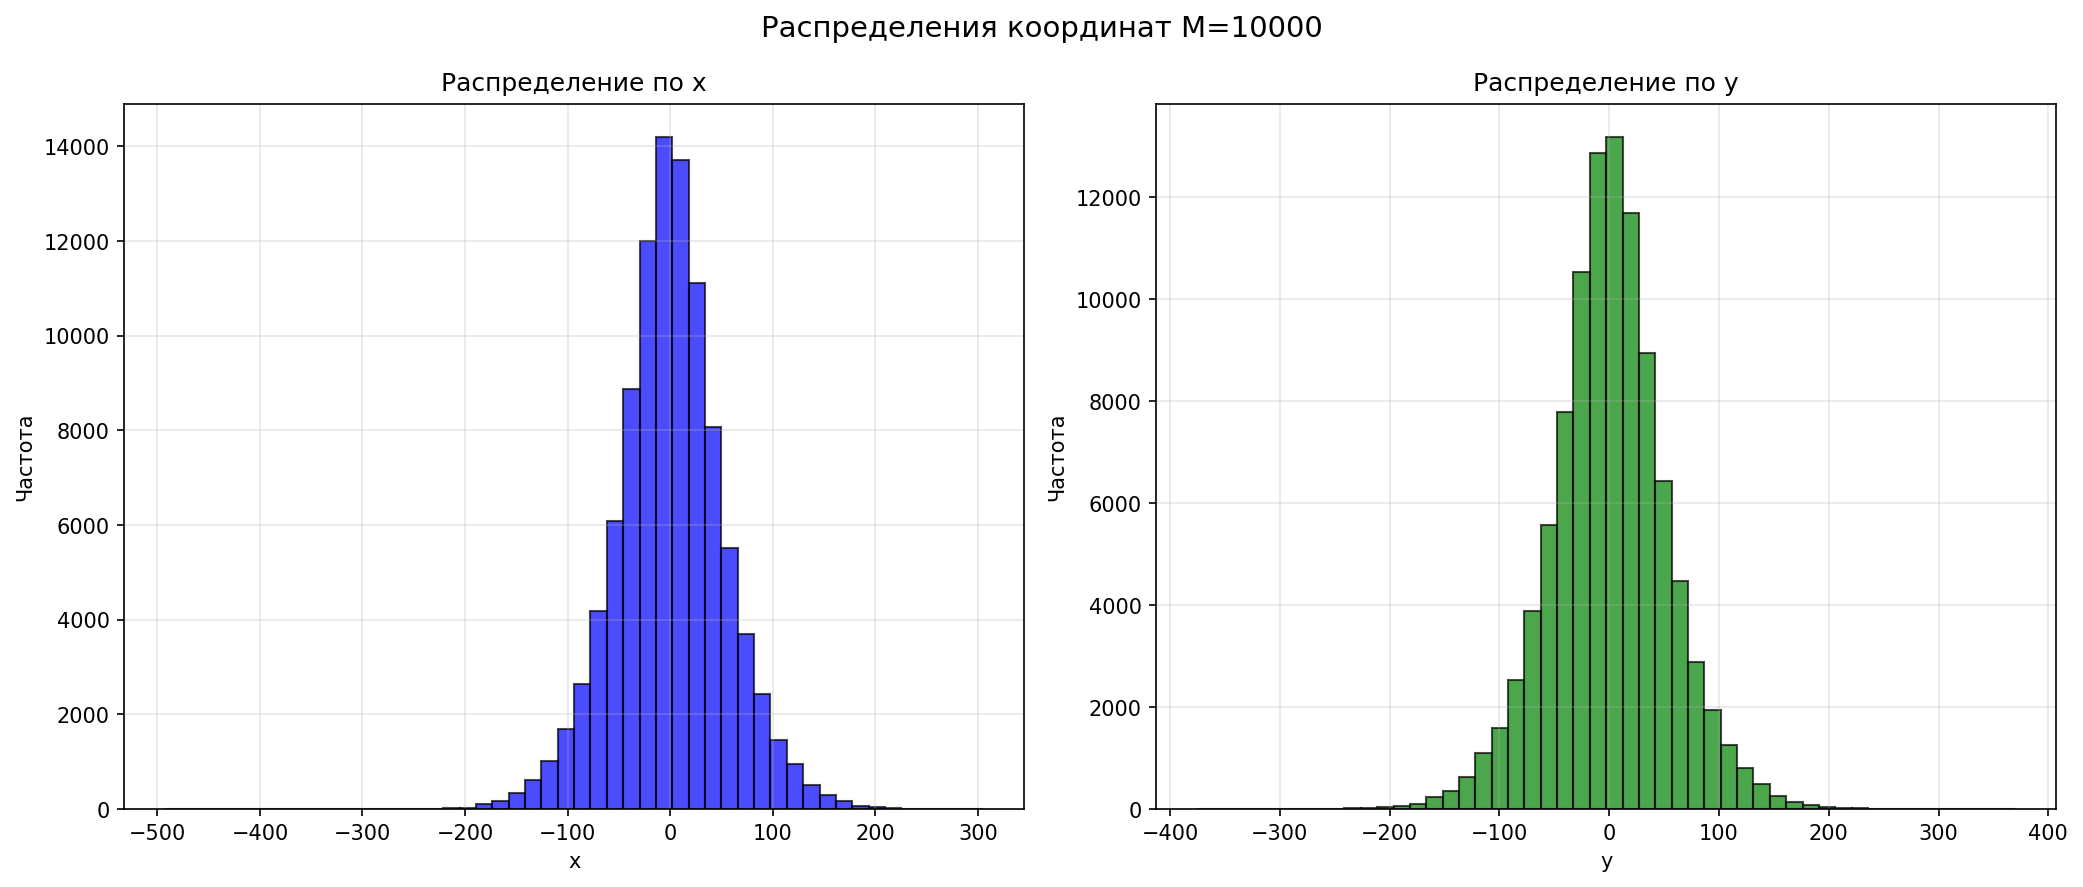
\includegraphics[width=1.0\linewidth]{../out/histograms_M10000}
		\caption{Гистограмма распределения M = 10000}
		\label{fig:histogramsm10000}
	\end{figure}
	
	\begin{figure}[H]
		\centering
		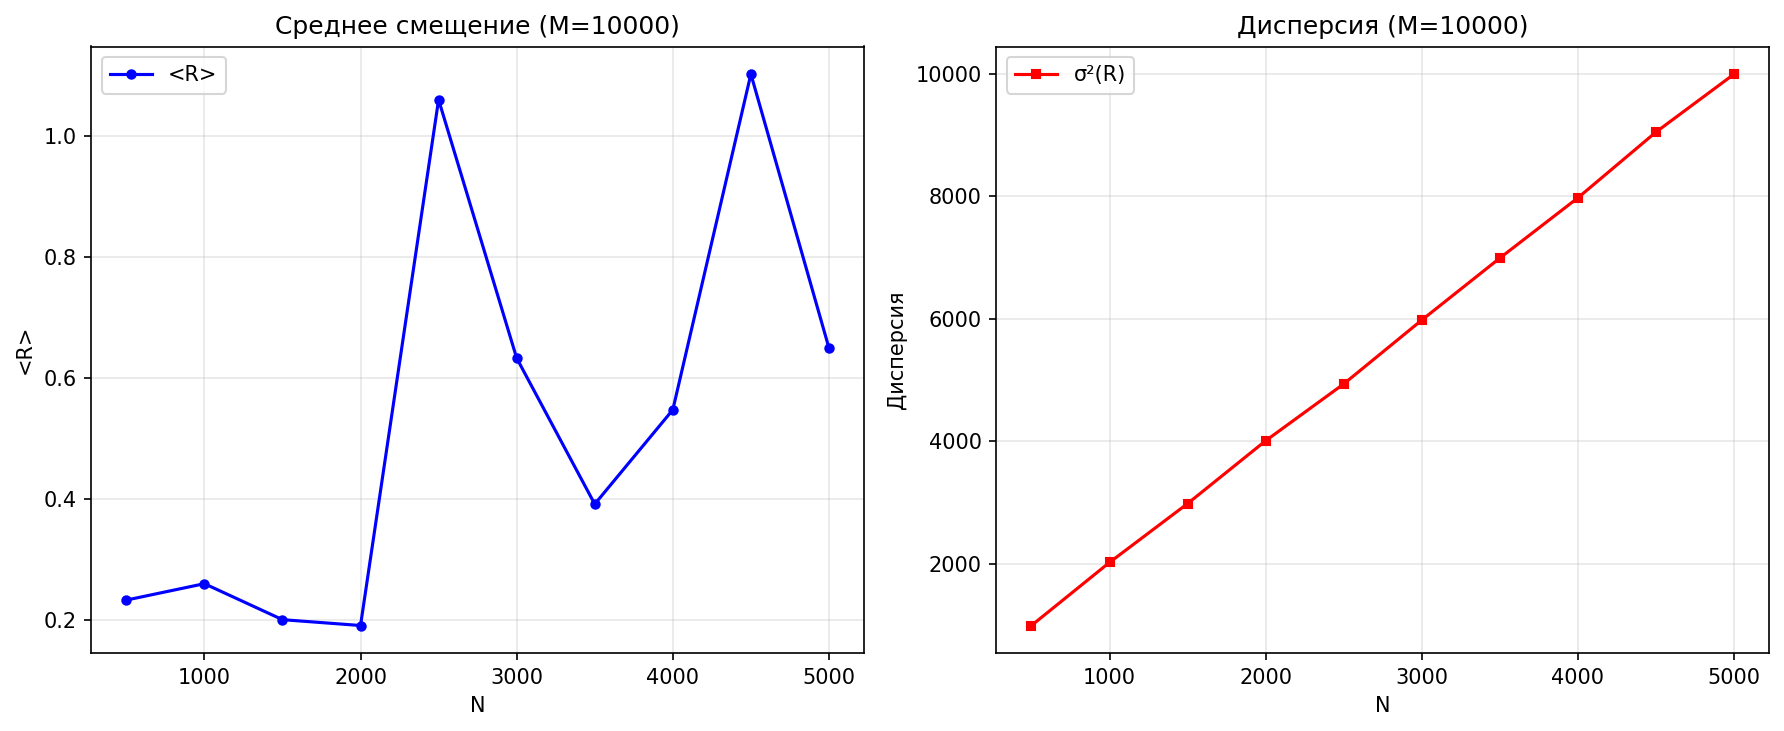
\includegraphics[width=1.0\linewidth]{../out/statistics_M10000}
		\caption{Статистика для распределения M = 10000}
		\label{fig:statisticsm10000}
	\end{figure}
	
	\subsection{Построение аппроксимации}
	
	При помощи метода наименьших квадратов построены аппроксимации ~\eqref{min_squares_condition}.
	
	\begin{figure}[H]
		\centering
		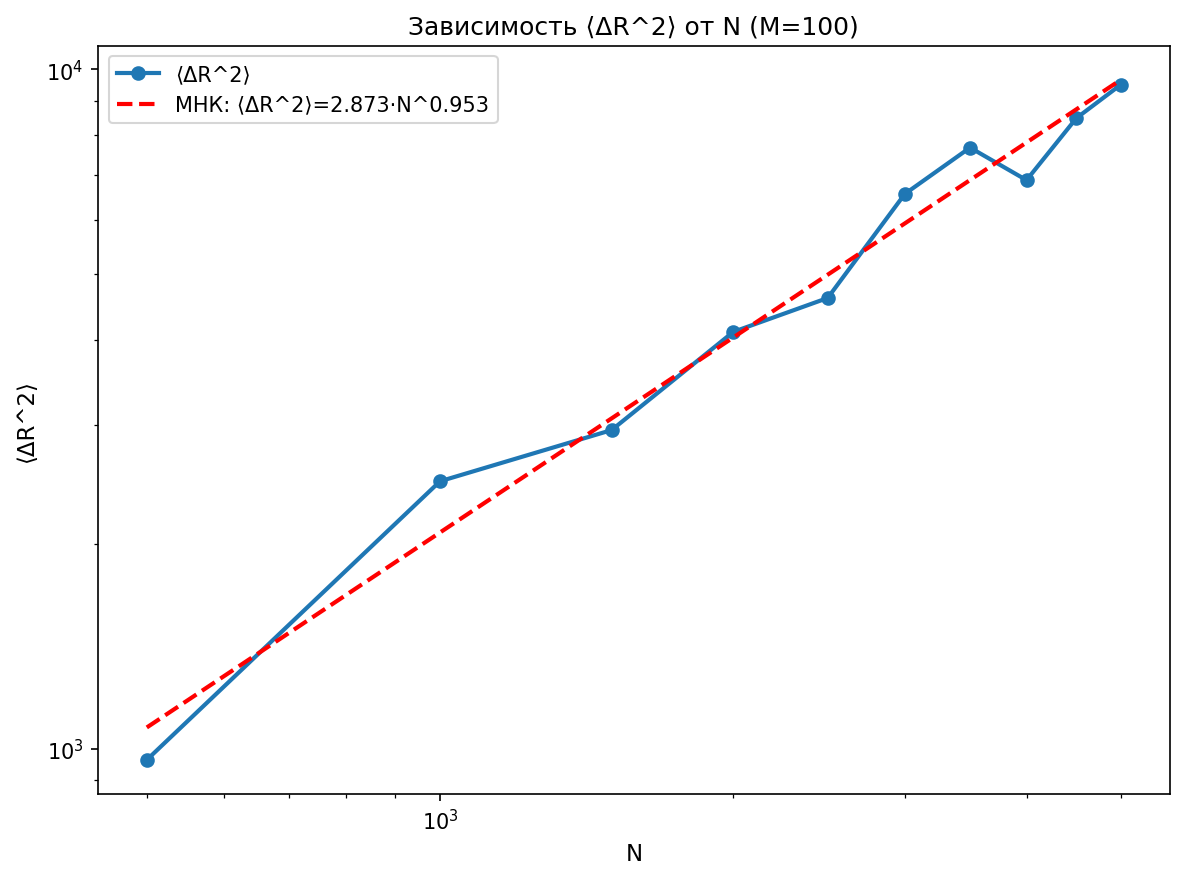
\includegraphics[width=0.8\linewidth]{../out/mnk_M100}
		\caption{Аппроксимация зависимости M = 100}
		\label{fig:mnkm100}
	\end{figure}
	
	\begin{figure}[H]
		\centering
		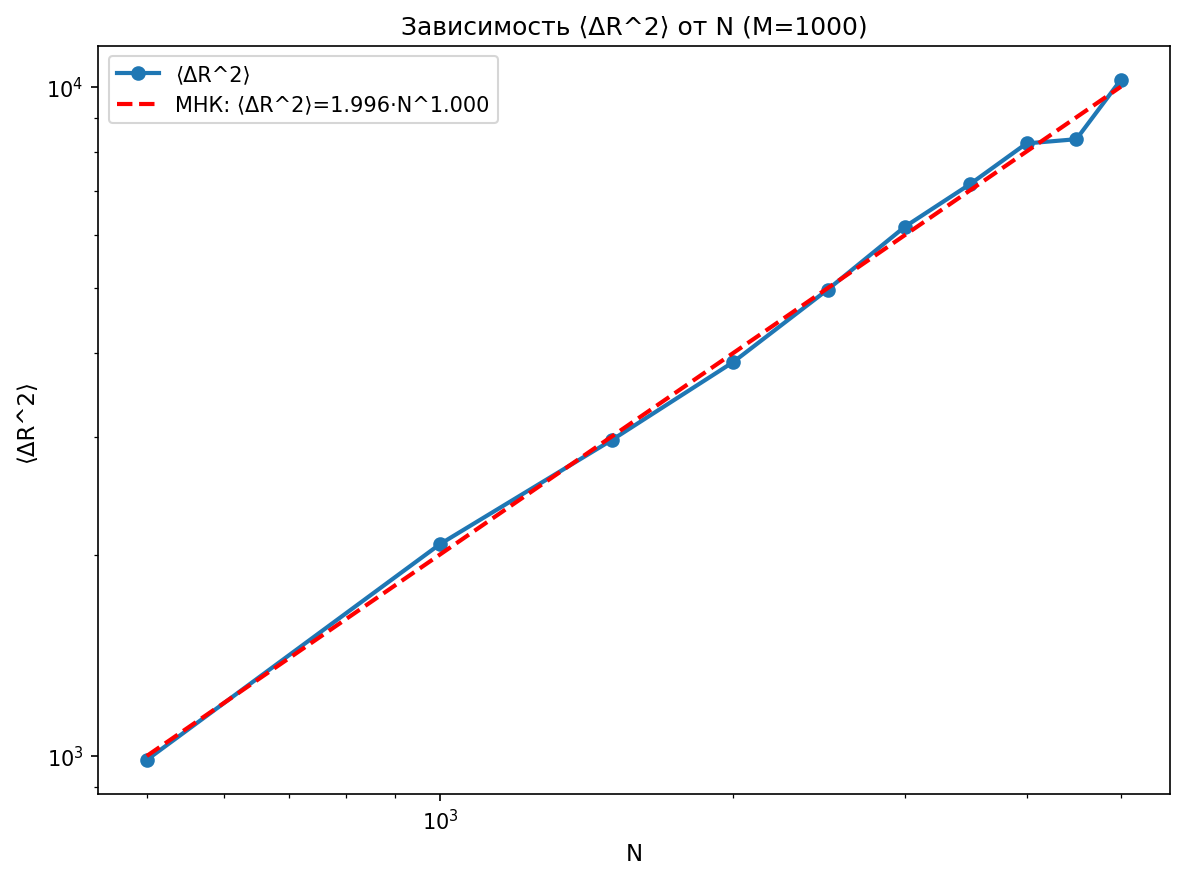
\includegraphics[width=0.8\linewidth]{../out/mnk_M1000}
		\caption{Аппроксимация зависимости M = 1000}
		\label{fig:mnkm1000}
	\end{figure}
	
	\begin{figure}[H]
		\centering
		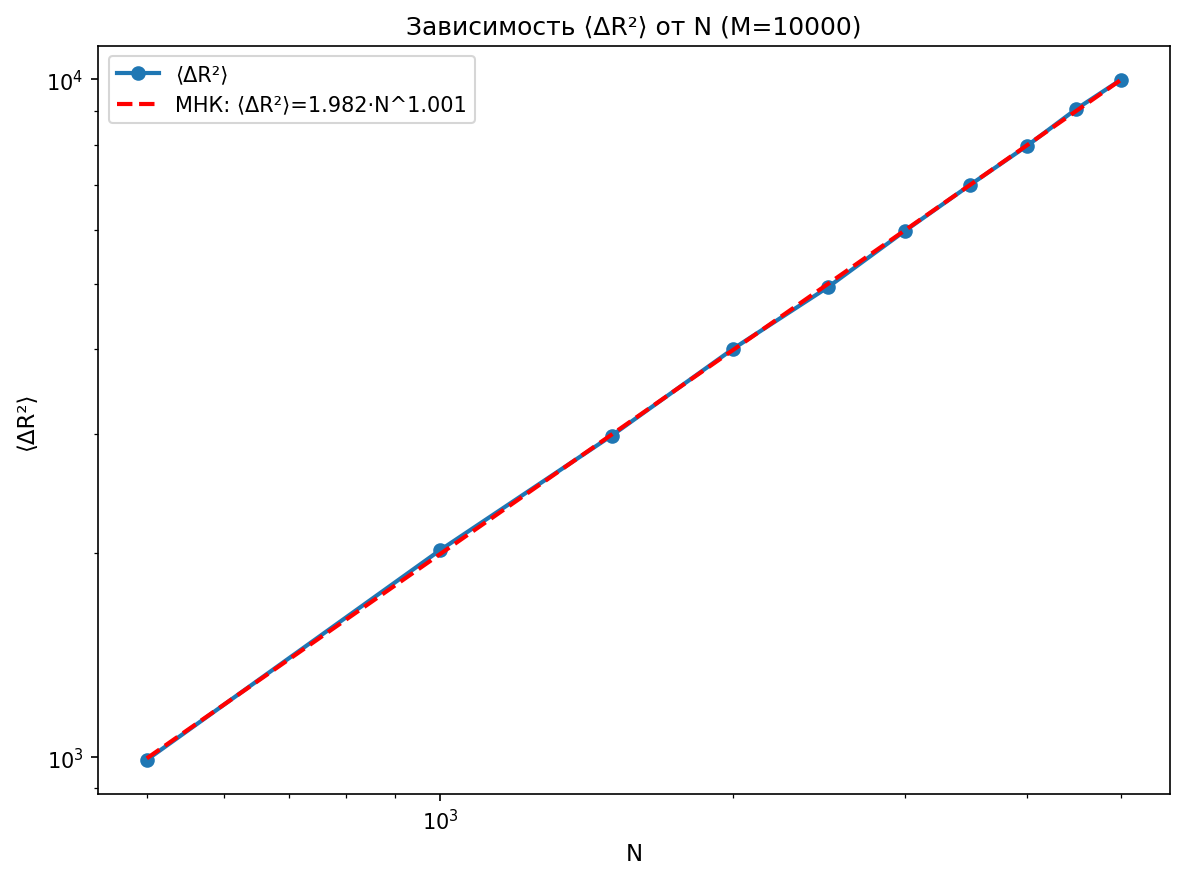
\includegraphics[width=0.8\linewidth]{../out/mnk_M10000}
		\caption{Аппроксимация зависимости M = 10000}
		\label{fig:mnkm10000}
	\end{figure}
	
	Полученные параметры аппроксимации представлены в таблице ~\ref{tab:result}.
	
	\begin{table}[h!]
		\centering
		\caption{Параметры аппроксимации}
		\label{tab:result}
		\renewcommand{\arraystretch}{1.5}
		\begin{tabular}{|c|c|c|c|p{4cm}|}
			\hline
			$M$ & $A$ & $\nu$ \\
			\hline
			100  & 2.473 & 0.980 \\
			\hline
			1000 & 1.497 & 1.039 \\
			\hline
			10000& 1.982 & 1.001 \\
			\hline
		\end{tabular}
	\end{table}
	
	Рассчитаем теоретические моменты распределения плотности ~\eqref{ifit_func}:
	
	\begin{equation}
		M_1 = \int_{0}^{\infty} l f(l) dl = 1.15,
		\nonumber
	\end{equation}
	\begin{equation}
		M_2 = \int_{0}^{\infty} l^2 f(l) dl = 2.
		\nonumber
	\end{equation}
	
	Полученные значения $\nu$ близки к единице, что соответствует нормальной диффузии. Теоретические моменты распределения конечны, что также указывает на применимость центральной предельной теоремы и нормальный характер диффузии. Таким образом, асимптотическое распределение частиц стремится к нормальному закону.
	
	\newpage
	\section{Вывод}
	
	В ходе лабораторной работы была реализована программа, моделирующая диффузионные процессы методом случайных блужданий. Из экспериментов установили, что распределения подчиняются нормальному закону.
	
	\newpage
	\section{Листинг}
	
	\begin{lstlisting}[title=main.cpp, gobble=16, breaklines=true, showspaces=false, showtabs=false, breakatwhitespace=true]
		#include <omp.h>
		#include <pybind11/embed.h>
		#include <pybind11/numpy.h>
		#include <pybind11/stl.h>
		
		#include <chrono>
		#include <cmath>
		#include <iostream>
		#include <random>
		#include <vector>
		
		namespace py = pybind11;
		
		struct Statistics {
			double mean_x, mean_y;
			double var_x, var_y;
			double var_R, mean_R;
			std::vector<double> x_coords, y_coords;
			std::vector<std::vector<double>> trajectories_x;
			std::vector<std::vector<double>> trajectories_y;
		};
		
		class RandomWalksVisualizer {
			private:
			const double PI = M_PI;
			
			public:
			double invert_func(double r) { return pow(tan(PI * r / 2.0), 1.0 / 3.0); }
			
			struct Trajectory {
				std::vector<double> x_coords;
				std::vector<double> y_coords;
			};
			
			Trajectory simulate_with_trajectory(int N, std::mt19937& rng) {
				Trajectory traj;
				traj.x_coords.reserve(N + 1);
				traj.y_coords.reserve(N + 1);
				
				double x = 0.0, y = 0.0;
				traj.x_coords.push_back(x);
				traj.y_coords.push_back(y);
				
				std::uniform_real_distribution<> dis(0.0, 1.0);
				std::uniform_int_distribution<> dir_dis(0, 3);
				
				for (int step = 0; step < N; step++) {
					double r = dis(rng);
					double length = invert_func(r);
					int direction = dir_dis(rng);
					
					switch (direction) {
						case 0:
						y += length;
						break;
						case 1:
						y -= length;
						break;
						case 2:
						x -= length;
						break;
						case 3:
						x += length;
						break;
					}
					
					traj.x_coords.push_back(x);
					traj.y_coords.push_back(y);
				}
				
				return traj;
			}
			
			std::vector<Trajectory> simulate_parallel_with_trajectories(int M, int N, int num_threads = 4) {
				if (num_threads > 0) {
					omp_set_num_threads(num_threads);
				}
				
				std::vector<Trajectory> results(M);
				
				#pragma omp parallel for
				for (int i = 0; i < M; i++) {
					std::mt19937 thread_rng(std::random_device{}() + omp_get_thread_num() * 12345);
					results[i] = simulate_with_trajectory(N, thread_rng);
				}
				
				return results;
			}
			
			Statistics compute_statistics_from_trajectories(const std::vector<Trajectory>& trajectories) {
				Statistics stats;
				int M = trajectories.size();
				
				stats.x_coords.reserve(M);
				stats.y_coords.reserve(M);
				stats.trajectories_x.reserve(M);
				stats.trajectories_y.reserve(M);
				
				double sum_x = 0.0, sum_y = 0.0;
				double sum_x2 = 0.0, sum_y2 = 0.0;
				
				for (const auto& traj : trajectories) {
					double x_final = traj.x_coords.back();
					double y_final = traj.y_coords.back();
					
					stats.x_coords.push_back(x_final);
					stats.y_coords.push_back(y_final);
					
					stats.trajectories_x.push_back(traj.x_coords);
					stats.trajectories_y.push_back(traj.y_coords);
					
					sum_x += x_final;
					sum_y += y_final;
					sum_x2 += x_final * x_final;
					sum_y2 += y_final * y_final;
				}
				
				stats.mean_x = sum_x / M;
				stats.mean_y = sum_y / M;
				stats.var_x = sum_x2 / M - stats.mean_x * stats.mean_x;
				stats.var_y = sum_y2 / M - stats.mean_y * stats.mean_y;
				stats.var_R = stats.var_x + stats.var_y;
				stats.mean_R = sqrt(stats.mean_x * stats.mean_x + stats.mean_y * stats.mean_y);
				
				return stats;
			}
			
			void send_to_python_and_plot(const std::vector<Trajectory>& trajectories, int M, int N,
			double elapsed_time) {
				Statistics stats = compute_statistics_from_trajectories(trajectories);
				
				py::array_t<double> x_coords(stats.x_coords.size());
				py::array_t<double> y_coords(stats.y_coords.size());
				
				auto x_buf = x_coords.request();
				auto y_buf = y_coords.request();
				
				double* x_ptr = static_cast<double*>(x_buf.ptr);
				double* y_ptr = static_cast<double*>(y_buf.ptr);
				
				for (size_t i = 0; i < stats.x_coords.size(); i++) {
					x_ptr[i] = stats.x_coords[i];
					y_ptr[i] = stats.y_coords[i];
				}
				
				py::list traj_x_list, traj_y_list;
				
				int num_trajectories_to_save = std::min(10, (int)trajectories.size());
				for (int i = 0; i < num_trajectories_to_save; i++) {
					py::list traj_x, traj_y;
					for (size_t j = 0; j < trajectories[i].x_coords.size(); j++) {
						traj_x.append(trajectories[i].x_coords[j]);
						traj_y.append(trajectories[i].y_coords[j]);
					}
					traj_x_list.append(traj_x);
					traj_y_list.append(traj_y);
				}
				
				py::dict data;
				data["x_coords"] = x_coords;
				data["y_coords"] = y_coords;
				data["trajectories_x"] = traj_x_list;
				data["trajectories_y"] = traj_y_list;
				data["mean_x"] = stats.mean_x;
				data["mean_y"] = stats.mean_y;
				data["var_x"] = stats.var_x;
				data["var_y"] = stats.var_y;
				data["var_R"] = stats.var_R;
				data["mean_R"] = stats.mean_R;
				data["M"] = M;
				data["N"] = N;
				data["time"] = elapsed_time;
				
				try {
					py::module_ plotter = py::module_::import("main");
					plotter.attr("plot_simulation_results")(data);
				} catch (const py::error_already_set& e) {
					std::cerr << "Python error: " << e.what() << std::endl;
				}
			}
			
			void run_with_visualization(const std::vector<int>& M_values, const std::vector<int>& N_values,
			int num_threads = 4) {
				try {
					py::module_::import("matplotlib");
					std::cout << "Matplotlib imported successfully\n";
				} catch (const py::error_already_set& e) {
					std::cerr << "Failed to import matplotlib: " << e.what() << std::endl;
					return;
				}
				
				for (int M : M_values) {
					for (int N : N_values) {
						std::cout << "M = " << M << ", N = " << N << std::flush;
						
						auto start = std::chrono::high_resolution_clock::now();
						
						auto trajectories = simulate_parallel_with_trajectories(M, N, num_threads);
						
						auto end = std::chrono::high_resolution_clock::now();
						double elapsed = std::chrono::duration<double>(end - start).count();
						
						std::cout << ", done in " << elapsed << "s" << std::endl;
						
						send_to_python_and_plot(trajectories, M, N, elapsed);
					}
				}
				
				try {
					py::module_ plotter = py::module_::import("main");
					plotter.attr("plot_summary_plots")();
				} catch (const py::error_already_set& e) {
					std::cerr << "Python error in summary: " << e.what() << std::endl;
				}
			}
		};
		
		int main(int argc, char* argv[]) {
			py::scoped_interpreter guard{};
			
			try {
				py::module_ sys = py::module_::import("sys");
				py::list path = sys.attr("path");
				
				path.attr("insert")(0, ".");
				
				std::string src_path = "/home/aigul/Documents/vs_code_projects/matmod/labs/lr4/src";
				path.attr("insert")(0, src_path);
				
				std::cout << "Python sys.path configured\n";
			} catch (const py::error_already_set& e) {
				std::cerr << "Failed to configure Python path: " << e.what() << std::endl;
			}
			
			RandomWalksVisualizer simulator;
			
			std::vector<int> M_values = {100, 1000, 10000};
			std::vector<int> N_values;
			for (int N = 500; N <= 5000; N += 500) {
				N_values.push_back(N);
			}
			
			simulator.run_with_visualization(M_values, N_values, 8);
			
			std::cout << "\nPress Enter to exit...";
			std::cin.get();
			
			return 0;
		}
	\end{lstlisting}
	

	\begin{lstlisting}[title=main.py, gobble=16, breaklines=true, showspaces=false, showtabs=false, breakatwhitespace=true]
		import matplotlib
		
		matplotlib.use("Agg")
		
		from pathlib import Path
		
		import matplotlib.pyplot as plt
		import numpy as np
		
		current_dir = Path(__file__).parent.absolute()
		project_root = current_dir.parent.parent.parent
		RESULTS_DIR = project_root / "labs/lr4/out"
		RESULTS_DIR.mkdir(exist_ok=True)

		all_results = {}
		
		def plot_simulation_results(data):
			M = data["M"]
			N = data["N"]
			x_coords = np.array(data["x_coords"])
			y_coords = np.array(data["y_coords"])
			trajectories_x = data["trajectories_x"]
			trajectories_y = data["trajectories_y"]
			mean_x = data["mean_x"]
			mean_y = data["mean_y"]
			var_x = data["var_x"]
			var_y = data["var_y"]
			var_R = data["var_R"]
			mean_R = data["mean_R"]
			
			if M not in all_results:
			all_results[M] = {}
			all_results[M][N] = {
				"x_coords": x_coords,
				"y_coords": y_coords,
				"trajectories_x": trajectories_x,
				"trajectories_y": trajectories_y,
				"mean_x": mean_x,
				"mean_y": mean_y,
				"var_x": var_x,
				"var_y": var_y,
				"var_R": var_R,
				"mean_R": mean_R,
			}
			
			if len(trajectories_x) > 0:
				plot_trajectory(trajectories_x[0], trajectories_y[0], M, N)
			plot_mnk_for_each_M()
		
		
		def plot_mnk_for_each_M():
			for M, results in all_results.items():
			N_values = sorted(results.keys())
			var_R_values = [results[N]["var_R"] for N in N_values]
			
			log_N = np.log(N_values)
			log_var = np.log(var_R_values)
			nu, ln_A = coeffs[0], coeffs[1]
			A = np.exp(ln_A)
			
			N_fit = np.linspace(min(N_values), max(N_values), 100)
			var_R_fit = A * N_fit**nu
			
			fig, ax = plt.subplots(figsize=(8, 6))
			ax.loglog(
				N_values,
				var_R_values,
				"o-",
				label="<\Delta R^2>",
				markersize=6,
				linewidth=2,
				)
				ax.loglog(
				N_fit, var_R_fit, "r--", label=f"MNK: <$\Delta$R>={A:.3f}*N^{nu:.3f}", linewidth=2
			)
			
			ax.set_xlabel("N", fontsize=11)
MHK			ax.set_ylabel("<delta R^2>", fontsize=11)
			ax.legend(fontsize=10)
			
			plt.tight_layout()
			filename = RESULTS_DIR / f"mnk_M{M}.png"
			plt.savefig(filename, dpi=150, bbox_inches="tight")
			plt.close(fig)
		
		
		def plot_trajectory(traj_x, traj_y, M, N):
			fig, ax = plt.subplots(figsize=(9, 8))
			
			ax.plot(traj_x, traj_y, "b-", linewidth=1.5, alpha=0.8)
			ax.plot(traj_x[0], traj_y[0], "go", markersize=6, label="Start")
			ax.plot(traj_x[-1], traj_y[-1], "ro", markersize=6, label="Finish")
			
			ax.set_xlabel("x")
			ax.set_ylabel("y")
			ax.set_title(f"First trajectory (M={M}, N={N})")
			ax.grid(True, alpha=0.3)
			ax.axis("equal")
			ax.legend(loc="upper right")
			
			plt.tight_layout()
			
			filename = RESULTS_DIR / f"trajectory_M{M}_N{N}.png"
			plt.savefig(filename, dpi=150)

			plt.close(fig)
		
		
		def plot_summary_plots():
			fig, ax = plt.subplots(figsize=(10, 6))
			for M, results in all_results.items():
				N_values = sorted(results.keys())
				var_R_values = [results[N]["var_R"] for N in N_values]
				ax.loglog(N_values, var_R_values, "o-", label=f"M={M}", markersize=6)
				
				if len(N_values) > 1:
					log_N = np.log(N_values)
					log_var = np.log(var_R_values)
					coeffs = np.polyfit(log_N, log_var, 1)
					nu = coeffs[0]
					A = np.exp(coeffs[1])
					theory = A * np.array(N_values) ** nu
					ax.loglog(N_values, theory, "--", alpha=0.5, label=f"M={M} (nu={nu:.3f})")
			

			ax.set_xlabel("N")
			ax.set_ylabel("<delta R^2>")
			ax.grid(True, alpha=0.3, which="both")
			ax.legend(fontsize=10)
			
			filename = RESULTS_DIR / "var_R_vs_N.png"
			plt.savefig(filename, dpi=150, bbox_inches="tight")
			plt.close(fig)
			

			for M, results in all_results.items():
				fig, axes = plt.subplots(1, 2, figsize=(12, 5))
				
				N_values = sorted(results.keys())
				mean_R_values = [results[N]["mean_R"] for N in N_values]
				var_R_values = [results[N]["var_R"] for N in N_values]
				
				axes[0].plot(
				N_values, mean_R_values, "o-", label="<R>", markersize=4, color="blue"
				)
				axes[0].set_xlabel("N")
				axes[0].set_ylabel("<R>")
				axes[0].grid(True, alpha=0.3)
				axes[0].legend()
				

				axes[1].plot(
					N_values, var_R_values, "s-", label="ro^2(R)", markersize=4, color="red"
				)
				axes[1].set_xlabel("N")
				axes[1].set_ylabel("Variance")
				axes[1].set_title(f"Variance (M={M})")
				axes[1].grid(True, alpha=0.3)
				axes[1].legend()
				
				plt.tight_layout()
				filename = RESULTS_DIR / f"statistics_M{M}.png"
				plt.savefig(filename, dpi=150, bbox_inches="tight")
				plt.close(fig)
			
			plot_histograms_for_each_M()
			
			
			def plot_histograms_for_each_M():
				for M, results in all_results.items():
					fig, axes = plt.subplots(1, 2, figsize=(14, 6))
					fig.suptitle(f"Frequency M={M}", fontsize=14)
					
					all_x_coords = []
					all_y_coords = []
					
					for N, stats in sorted(results.items()):
					all_x_coords.extend(stats["x_coords"])
					all_y_coords.extend(stats["y_coords"])
					
					all_x_coords = np.array(all_x_coords)
					all_y_coords = np.array(all_y_coords)
					
					total_mean_x = np.mean(all_x_coords)
					total_std_x = np.std(all_x_coords)
					total_mean_y = np.mean(all_y_coords)
					total_std_y = np.std(all_y_coords)
					
					ax1 = axes[0]
					n_x, bins_x, patches_x = ax1.hist(
						all_x_coords,
						bins=50,
						alpha=0.7,
						color="blue",
						edgecolor="black",
						linewidth=1,
					)
					ax1.set_xlabel("x")
					ax1.set_ylabel("Frequency")
					ax1.set_title("Distribution by x")
					ax1.grid(True, alpha=0.3)
					
					ax2 = axes[1]
					n_y, bins_y, patches_y = ax2.hist(
						all_y_coords,
						bins=50,
						alpha=0.7,
						color="green",
						edgecolor="black",
						linewidth=1,
					)
					ax2.set_xlabel("y")
					ax2.set_ylabel("Frequency")
					ax2.set_title("Distribution by y")
					ax2.grid(True, alpha=0.3)
					
					plt.tight_layout()
					filename = RESULTS_DIR / f"histograms_M{M}.png"
					plt.savefig(filename, dpi=150, bbox_inches="tight")
					print(
					f"M={M}: mean_x={total_mean_x:.4f}, std_x={total_std_x:.4f}, mean_y={total_mean_y:.4f}, std_y={total_std_y:.4f}"
					)
					plt.close(fig)
		
	\end{lstlisting}
	
\end{document}